\documentclass{article}

% if you need to pass options to natbib, use, e.g.:
%     \PassOptionsToPackage{numbers, compress}{natbib}
% before loading neurips_2021

% this year
\usepackage[]{neurips_2021_ml4ps}

% to compile a preprint version, e.g., for submission to arXiv, add add the
% [preprint] option:
%     \usepackage[preprint]{neurips_2021}

% to compile a camera-ready version, add the [final] option, e.g.:
%     \usepackage[final]{neurips_2021}

% to avoid loading the natbib package, add option nonatbib:
%    \usepackage[nonatbib]{neurips_2021}

\usepackage[utf8]{inputenc} % allow utf-8 input
\usepackage[T1]{fontenc}    % use 8-bit T1 fonts
\usepackage{graphicx}
\usepackage[colorlinks=true, allcolors=blue]{hyperref}
\usepackage[]{todonotes}
%\usepackage{hyperref}       % hyperlinks
\usepackage{url}            % simple URL typesetting
\usepackage{booktabs}       % professional-quality tables
\usepackage{nicefrac}       % compact symbols for 1/2, etc.
\usepackage{microtype}      % microtypography
\usepackage{xcolor}         % colors
\usepackage{enumitem}
\usepackage{bm}
\usepackage{amsmath}
\usepackage{amsfonts}       % blackboard math symbols
\usepackage{latexsym}
\usepackage{amssymb}
\usepackage{bbm}
\usepackage{mathrsfs}       % mathscr
%\usepackage[pdftex]{graphicx}
\usepackage{natbib}
\usepackage{comment}
\usepackage{caption} % subfigures
\usepackage{subcaption} % subfigures
\usepackage{wrapfig}
\usepackage[normalem]{ulem} % strikeout
\bibliographystyle{plain}

%% Handy macros and abbreviations
\newcommand\numberthis{\addtocounter{equation}{1}\tag{\theequation}}
\newcommand{\danm}[1]{\todo[inline,color=green!20!white]{\textbf{DanM:} #1}}
\newcommand{\danp}[1]{\todo[inline,color=blue!20!white]{\textbf{DanP:} #1}}
\newcommand{\petra}[1]{\todo[inline,color=yellow!20!white]{\textbf{Petra:} #1}}
\newcommand{\david}[1]{\todo[inline,color=orange!20!white]{\textbf{David:} #1}}
\newcommand{\var}{\operatorname{Var}}
\newcommand{\corr}{\operatorname{Corr}}
\newcommand{\dd}{\mathrm{d}}
\newcommand{\bb}[1]{\mathbb{#1}}
\newcommand{\vv}[1]{\boldsymbol{#1}}
\newcommand{\mm}[1]{\mathrm{#1}}
\newcommand{\rv}[1]{\mathsf{#1}}
\newcommand{\vrv}[1]{\vv{\rv{#1}}}
\newcommand{\dist}[1]{\mathcal{#1}}
\newcommand{\set}[1]{#1}
\newcommand{\op}[1]{\mathscr{#1}}
\newcommand{\unseen}[1]{\mm{P}_{u}#1}
\newcommand{\seenstate}[1]{\mm{P}_{x}{#1}}
\newcommand{\seeninp}[1]{\mm{P}_{u}{#1}}
\newcommand{\disteq}{\stackrel{\mathrm{d}}{=}}
\newcommand{\gvn}{\mid}
\newcommand{\Ex}{\mathbb{E}}
\renewcommand{\Pr}{\mathbb{P}}
\newcommand{\solop}{\mathcal{G}^{\dagger}}
\newcommand{\lat}{\rv{b}}   % Kept changing the symbol for latent state
\newcommand{\latst}{b}      % so now it is a macro
\newcommand{\latsp}{\mathcal{B}}
\newcommand{\inp}{\rv{u}}
\newcommand{\inpst}{u}
\newcommand{\inpsp}{\mathcal{U}}
\newcommand{\state}{\rv{x}}
\newcommand{\statest}{x}
\newcommand{\statesp}{\mathcal{X}}
\newcommand{\outp}{\rv{y}}
\newcommand{\outpst}{y}
\newcommand{\outpsp}{\mathcal{Y}}
\newcommand{\latwt}{\vrv{w}}
\newcommand{\latwtst}{\vv{w}}
\newcommand{\param}{\vrv{\theta}}  % misc param
\newcommand{\paramst}{\vv{\theta}}
% \newcommand{\hatlatents}{\widehat{\lat}_{\boldsymbol{\kappa}}}
\newcommand{\boundaries}{\vv{\phi}}

\title{Bayesian Model Inversion for Spatio-temporal Processes using surrogate operators}

% The \author macro works with any number of authors. There are two commands
% used to separate the names and addresses of multiple authors: \And and \AND.
%
% Using \And between authors leaves it to LaTeX to determine where to break the
% lines. Using \AND forces a line break at that point. So, if LaTeX puts 3 of 4
% authors names on the first line, and the last on the second line, try using
% \AND instead of \And before the third author name.

\author{%
  Dan MacKinlay\\
  CSIRO Data61\\
  \texttt{dan.mackinlay@data61.csiro.au} \\
  % examples of more authors
   \And
   Dan Pagendam \\
   CSIRO Data61 \\
  \texttt{dan.pagendam@data61.csiro.au} \\
   \And
   Petra M. Kuhnert \\
   CSIRO Data61 \\
   \texttt{petra.kuhnert@data61.csiro.au} \\
   Sreekanth Janardhanan\\
   CSIRO Land and Water \\
   \texttt{sreekanth.janardhanan@csiro.au} \\
}

\begin{document}

\maketitle

\begin{abstract}

\end{abstract}

Recent developments in operator approximation with neural nets have produced a high-performance family of networks that can robustly predict future states of a function-valued dynamical system, including U-Net \cite{RonnebergerUNet2015} and Fourier Neural Operators \cite{LiFourier2020,KovachkiNeural2021}.
As yet, there are few attempts to analyze the effectiveness of these models in the more challenging \emph{inverse} setting \cite{MacKinlayModel2021}.
Here we conduct a study of the effectiveness of the Fourier Neural Operator construction against the original model in terms of the accuracy and computational efficiency on solving inverse problems.


 \subsection{Posterior sampling by Stochastic Gradient descent}

\cite{MandtStochastic2017} gives conditions for approximation of the posterior distribution of a target RV by gradient descent.
Observe that the stochastic gradient is a sum of \(S\) independent, uniformly sampled contributions. Invoking the central limit theorem, we assume that the gradient noise is Gaussian with covariance \(\frac{1}{S} C(\theta)\), hence
\[
\hat{g}_S(\theta) \approx g(\theta)+\frac{1}{\sqrt{S}} \Delta g(\theta), \quad \Delta g(\theta) \sim \mathcal{N}(0, C(\theta)) .
\]
We assume that the covariance matrix \(C(\theta)\) is approximately constant with respect to \(\theta\).
As a symmetric positive-semidefinite matrix, this constant matrix \(C\) factorizes as
\[
C(\theta) \approx C=B B^{\top}
\]
We approximate SGD as an Ornstein-Uhlenbeck process.
\[
d \theta(t)=-\epsilon A \theta(t) d t+\frac{1}{\sqrt{S}} \epsilon B d W(t)
\]
The Ornstein-Uhlenbeck process has a Gaussian analytic stationary distribution \(q(\theta)\).
\[
q(\theta) \propto \exp \left\{-\frac{1}{2} \theta^{\top} \Sigma^{-1} \theta\right\} .
\]
The covariance \(\Sigma\) satisfies
\[
\Sigma A+A \Sigma=\frac{\epsilon}{S} B B^{\top}
\]
Using their Theorem 2, The preconditioner for constant SGD that minimizes KL divergence from the stationary distribution to the posterior is
\[
H^*=\frac{2 S}{N}\left(B B^{\top}\right)^{-1}
\]

We can use this if we can cheaply calculate \((\mm{B}\mm{B}^{\top})^{-1}\) s.t.
\begin{align*}
\mm{B}\mm{B}^{\top}
    &=\mm{C}\\
    &= \var\left[\nabla_{\theta}\mathcal{L}\right]\\
    &= \Ex\left[\nabla_{\theta}\mathcal{L}\nabla_{\theta}^{\top}\mathcal{L}\right]
    - \Ex\left[\nabla_{\theta}\mathcal{L}\right]\Ex\left[\nabla_{\theta}^{\top}\mathcal{L}\right]\\
    &= \Ex\left[\nabla_{\theta}\mathcal{L}\nabla_{\theta}^{\top}\mathcal{L}\right] &\text{opt}\\
    &\simeq \Ex\left[\nabla^2_{\theta}\mathcal{L}\right] &\text{Fisher}\\
    &= \mm{K}_{\theta\theta}^{-1} \gvn\mathcal{D} &\text{Gaussian}
\end{align*}
Have I inverted something? looks like we have a trivial preconditioner of the gradients.
Also where did prior go?


\subsection{Operator inversion by spatial belief propagation}

Suppose we partition the size in the unobserved field and propagate updates between them.
Can we marginalize out the observations and propagate updates?

Partition \(\forcing\) into \(\forcing\) and \(\forcing^{*}\).
The joint finite-dimensional distributions are
\begin{align*}
\left[\begin{array}{c}
    \tilde{\vv{\state}}_{t} \\
    \tilde{\forcing}\\
    \tilde{\forcing}^{*}
\end{array}\right]
&\sim\dist{N}\left(
    \left[\begin{array}{c}
        \vv{m}_{\tilde{\vv{\state}}_{t}}\\
        \vv{m}_{\tilde{\forcing}}\\
        \vv{m}_{\tilde{\forcing}^{*}}
    \end{array}\right],
    \left[\begin{array}{ccc}
        \mm{K}_{\tilde{\vv{\state}}_{t}\tilde{\vv{\state}}_{t}}
        & \mm{K}_{\tilde{\vv{\state}}_{t}\tilde{\forcing}}^{\top}
        & \mm{K}_{\tilde{\vv{\state}}_{t}\tilde{\forcing}^{*}}^{\top} \\
          \mm{K}_{\tilde{\vv{\state}}_{t}\tilde{\forcing}}
        & \mm{K}_{\tilde{\forcing}\tilde{\forcing}}^{\top}
        & \mm{K}_{\tilde{\forcing}\tilde{\forcing}^{*}}^{\top} \\
          \mm{K}_{\tilde{\vv{\state}}_{t}\tilde{\forcing^{*}}}
        & \mm{K}_{\tilde{\forcing}\tilde{\forcing}^{*}}^{\top}
        & \mm{K}_{\tilde{\forcing^{*}}\tilde{\forcing}^{*}} \\
    \end{array}\right]\numberthis\label{eq:discrete_joint_naive_sub}
\right).
\end{align*}
Conditioning on \(\tilde{\vv{\state}}_{t},\tilde{\forcing}\),
\begin{align*}
    \tilde{\forcing}^{*}\gvn  \tilde{\vv{\state}}_{t},\tilde{\forcing}
&\sim\dist{N}(
    \hat{\vv{m}}_{\tilde{\forcing}^{*}},
    \hat{\mm{K}}_{\tilde{\forcing}^{*}\tilde{\forcing}^{*}}
).
\end{align*}
where
\begin{align*}
\hat{\vv{m}}_{\tilde{\forcing}^{*}}
&=\vv{m}_{\tilde{\forcing}^{*}} + \\
&\sim\dist{N}\left(
    \left[\begin{array}{c}
        \vv{m}_{\tilde{\vv{\state}}_{t}}\\
        \vv{m}_{\tilde{\forcing}}\\
        \vv{m}_{\tilde{\forcing}^{*}}
    \end{array}\right],
    \left[\begin{array}{ccc}
        \mm{K}_{\tilde{\vv{\state}}_{t}\tilde{\vv{\state}}_{t}}
        & \mm{K}_{\tilde{\vv{\state}}_{t}\tilde{\forcing}}^{\top}
        & \mm{K}_{\tilde{\vv{\state}}_{t}\tilde{\forcing}^{*}}^{\top} \\
          \mm{K}_{\tilde{\vv{\state}}_{t}\tilde{\forcing}}
        & \mm{K}_{\tilde{\forcing}\tilde{\forcing}}^{\top}
        & \mm{K}_{\tilde{\forcing}\tilde{\forcing}^{*}}^{\top} \\
          \mm{K}_{\tilde{\vv{\state}}_{t}\tilde{\forcing^{*}}}
        & \mm{K}_{\tilde{\forcing}\tilde{\forcing}^{*}}^{\top}
        & \mm{K}_{\tilde{\forcing^{*}}\tilde{\forcing}^{*}} \\
    \end{array}\right]\numberthis\label{eq:discrete_joint_naive_sub}
\right).
\end{align*}

\subsection{Posterior sampling using instrumental variable approximate Bayesian neural operators}

When does a neural network ever imply anything about its own inputs?
Classic ProbNNs have this structure
\begin{align*}
    \vrv{y}=f(\vrv{x}, \vrv{w}, \netparamst)
\end{align*}
where by assumption \(\vrv{x} \indep \vrv{w}\) at inference time (i.e.
\(\vrv{x},\vrv{y} \indep \vrv{w}\gvn\mathcal{D}\).
This is probably fine for calculating a posterior predictive.
However, it can be problematic for inverting the model, since means that the weights \(\vrv{w}\) are not informative about network inputs.
If we wish to have a network which is probabilistically invertible we need to introduce some kind of model for a conditional dependence \(\vrv{w}\gvn\vrv{x}\).
The simplest such model would be to assume an auxiliary network \(\Ex\vrv{w}=g(\vrv{x})\), and maintaining the (contrived) assumption that this does not affect the conditional covariance.
If everything worked very nicely this might give us a consistent means of introducing coupling such that the weights were informative about the model inputs.

The combined network with params written explicitly is then
\begin{align*}
    \vrv{y} &=f(\vrv{x}, \vrv{w}, \netparamst) \\
    \vrv{w} & \sim \dist{N}\left(g(\vrv{x}, \vv{\psi}), \Sigma_{\vv{w}}\right)
\end{align*}
where \(\netparamst, \vv{\psi} \) are point-estimated by gradient descent, and \(\Sigma_{\vv{w}}\) is learned by conditioning a variational approximation.

Why bother?
The nice thing is that we can then update samples \(\vrv{x}\gvn\vrv{w}\), I think.
If the model graph comes out OK can we

\section{Questions and notes}

\begin{itemize}
    \item Is this model of observing a discrete sites ideal? should we be measuring some kind of inner-product representation in some Hilbert space?
    \item Idea: Random Fourier feature difference?
\end{itemize}

\subsection{How to represent a posterior Gaussian field tractably}

\begin{itemize}
    \item GP in some basis
    \begin{itemize}
        \item lattice/ FEM grid.
        \item fourier+canonical basis for posterior updates
    \end{itemize}
    \item Sparse GP, learn inducing points to approximate implied distributions of data.
    \item Normalising flow/ measure transport - learns a new neural net for each problem, direct Wasserstein inference under Gaussian approx.
    \item SWAG
    \item \sout{plain Gauss-Newton step} still need large inverse
    \item natural gradient
    \item GBP
    \item \sout{Need to learn what INLA is in case I re-invented it}
    \item Bayes matrix completion?
\end{itemize}

\listoftodos

\section{Operator inversion}

We briefly recap the theory of solving inverse problems using a forward predictor.
Suppose we have a deterministic prediction operator,
\(\op{P}:\statesp\times  \inpsp \to \statesp\) that maps from forcing space \( \inpsp\) and state space \(\statesp\) to state space \(\statesp\).\todo{we want to constrain these spaces or operators at all?} where of \(\statesp,\inpsp\) is a function space.\todo{over some domain which is compact subset of \(\mathbb{R}^d\)? Except we also allow basis representation}
The prediction operator applied recursively defines a time series,\footnote{In this work we consider the case of a static forcing, but extension to time-varying \(\inpst\) is straightforward}
\begin{align*}
    \statest_{t}=\op{P}(\statest_{t-1}, \inpst).
\end{align*}
In the forward problem our goal is construct predictions for each successive timestep with low error.
In the inverse setting, we observe the forcing and state inputs only through projections \(\seenstate{}: \statesp \to \mathbb{R}^{d_\state},\seeninp{}: \inpsp \to \mathbb{R}^{d_\inp},\).
The goal, given a series of observations comprised of projections of the observations, \(\set{D}:=\{\seenstate{\statest}_{1},\dots, \seenstate{\statest}_{T},\seeninp{\inpst}\}\), is to estimate the complete data
\(\{\statest_{1},\dots, \statest_{T},\inpst_{T}\}\)
such that the estimates \(\{\hat{\statest}_{1},\dots,\hat{\statest}_{T},\hat{\inpst}\}\), taken as inputs to the recursive prediction operator, reconstruct the observations with low error by some metric, i.e. that for \(t=2,\dots,T\),
\(\seenstate{\statest}_{t}\approx\seenstate{\op{P}}\left(\hat{\statest}_{t-1}, \hat{\inpst}\right)\) and \(\seeninp{\inpst}\approx\seeninp{\hat{\inpst}}\).\todo{representing the function in terms of some arbitrary basis still involves a projection step}

This problem is typically underdetermined, in the sense that many solutions may produce solutions with similar discrepancy from the observations.
This underdetermination can lead to various difficulties;
Optimisation may be unstable or ill-condition\todo{terminology?}; and there may be a difficulties in identifying and representing the entire feasible solution set.
The former problem is typically addressed by regularisation, favouring solutions which are closer to some plausible domain.
The latter is often addressed by maintaining ensembles of possible solutions.
Probabilistic methods address both challenges, simultaneously regularizing solutions via a prior measure on the solution function space and estimating a distribution over the set of feasible solutions.
\begin{comment}
Dan: You may be interested to have a look at Tikhonov (and singular value decomposition) regularisation method as described in the PEST book (I will send you on teams). These are quite popular in the groundwater model calibration and uncertainty analysis world.
\end{comment}
The probabilistic model assigns distributions to various quantities of interest, e.g.
\begin{align*}
\state_{t} \gvn \state_{t-1},\inp
&= \op{P}(\state_{t-1},\inp ), \quad t=2,\dots,T.
\numberthis \label{eq:proc_proj_sem} \\
\state_{t}
&\sim \dist{X}\\
\inp & \sim \dist{U}.
\end{align*}
The task is then to infer
\begin{align*}
\left(\state_{1},\dots, \state_{T},\inp \right)\gvn
\left(\seenstate{\state}_{1},\dots, \seenstate{\state}_{T},\seeninp{\inp}\right)
\numberthis \label{eq:proc_proj_sem_inv}
\end{align*}

For convenience we assume priors likley to lead to tractable computations.
Here we consider\todo{multidimensional output space?}
\begin{align*}
\state &\sim \dist{GP}(m_{\state},k_{\state}).
\numberthis \label{eq:gp_approx_state} \\
\inp &\sim \dist{GP}(m_{\inp},k_{\inp}).
\numberthis \label{eq:gp_approx_prior}
\end{align*}
The forward predictors we are interested in are one-step-ahead prediction operators arising from the governing equations of fluid flow and as such they are generally both nonlinear and computationally expensive, and the integrals involved in calculating the full conditional \eqref{eq:proc_proj_sem_inv} are analytically intractable.
We may however, approximate the posterior distribution by a Gaussian process also,\todo{in which metric?}
\begin{align*}
    \state_{t} \gvn \state_{t-1},\inp
&\sim \dist{GP}(\op{P}(\state_{t-1},\inp ), \op{K}(\state_{t-1},\inp )).
\numberthis \label{eq:gp_approx_proc}
\end{align*}
The posterior distributions in this case are still non-Gaussian in general.
We approximate the distributions over these solutions using collection of Monte Carlo samples from the relevant posterior distribution.
Estimating the posterior distribution of solutions via sampling \cite{EvensenData2009,TarantolaInverse2005}.

Mean predictor Monte Carlo treats the forward model as a mean predictor, assigns a Gaussian prior to the state and input parameters.
The posterior in this case is no longer Gaussian but is represented by samples.

Generalised Ensemble Kalman filtering updates an ensemble of samples from the target distribution to \dots

\section{Neural operator learning}

\section{Cheap model inversion using Bayesian Neural Operators}

Simulate from the neural linear model posterior

\section{Error analysis}


\section{Let's invert a neural net operator}

Model for process state evolution and observation.\footnote{Notation: We write random variates as sans-serif, \(\rv{x}\). When a function maps between function spaces, i.e. it is an operator, we emphasize this by writing it in  fraktur, \(\mathfrak{f}\). Both function spaces and sets are written calligraphically \(\mathcal{C}\).}
\begin{align*}
\rv{v}_{t} \gvn \lat, \rv{v}_{t-1}, \rv{v}_{t-2}, \dots
&\sim \dist{P}(\lat, \rv{v}_{t-1}, \rv{v}_{t-2}, \dots  )
\numberthis \label{eq:proc_sem} \\
\rv{y}_{t}\gvn \rv{v}_{t}
&\sim \dist{O}(\rv{v}_{t})\\
\lat & \sim \dist{T}.
\end{align*}
Usually we choose \(\Ex {\rv{y}_{t}} = \rv{v}_{t}\).

Here the solutions for \(\rv{v}_{t}\), are functions on some spatial domain \(\mathscr{S}\to\mathbb{R}\), say \(\mathscr{S}\subset \mathcal{R}^2\) and are all assumed exist a.s. in some function space \(v_t\in\set{V}\).
Similarly, the latent parameters are functions on the same domain \(\mathscr{S}\to\mathbb{R}\) in some possibly-different function space \(\latsp\), and the \(\rv{u}_{t}\) functions may exist in some other function space again.

Hereafter we suppress \(\rv{u}_{t}\), since they change little about the structure of the problem and add greatly to the clutter.

The goal: Can we infer a posterior distribution for
\(\lat\gvn\rv{y}_{t},\rv{y}_{t-1},\dots\) given some observations?

To keep the notation clean, we consider a simpler model which assumes only one time step of process history dependence (Figure~\ref{fig:filteringfgnoisy})
\begin{align*}
\rv{v}_{t}  \gvn \lat,\rv{v}_{t-1},
&\sim \dist{P}(\lat,\rv{v}_{t-1})
\numberthis \label{eq:proc_sem_lite} \\
\rv{y}_{t}  \gvn \rv{v}_{t}
&\sim \dist{O}(\rv{v}_{t}).
\end{align*}
Everything here should generalise to dependencies on multiple previous timesteps \todo{if the \(\rv{v}_{t-k}\) are observed, at least; not sure what happens more generally}

\subsection{Finite dimensional observations}
Thus far we have discussed distributions over functions only; we move to finite dimensional likelihoods by evaluating function values at some generic vector of test sites \(\set{S}:[\vv{x}_{i}]_{i}, i=1,\dots,M\).
To emphasise which function is evaluated at these sites, we use curly braces to suggest arguments that parameterise a function-valued mapping, so \(\op{f}\{y\}\) is a function parameterised by some (possibly function-valued) \(y\).
We use parentheses to suggest the evaluation of a function as usual, but for ordered-set-valued arguments we will assume the result is an vector function at some set of test points, so that \(\op{f}\{y\}(\set{S})\) is to be interpreted as the vector of point evaluations \(\op{f}\{y\}(x), x\in \set{S}\) of the function \(\op{f}\{y\}(\cdot)\).\todo{switch to projection operator as per \cite{LassasDiscretizationinvariant2009}?}
Analogously, we take \(\op{f}\{y\}(\set{S},\set{Y})\) to be the matrix of pairwise evaluations \([\op{f}\{y\}(\set{S},\set{Y})]_{i,j}, (x_i,y_j)\in\set{S}\times\set{Y}\).

Thus we can discuss the distribution of \(\rv{v}_{t}\gvn \lat,\rv{v}_{t-1}\) in terms of finite-dimensional moments,
\begin{align*}
\Ex[\rv{v}_{t}(\set{S})\gvn \lat,\rv{v}_{t-1}]
&= \op{P}\{\lat,\rv{v}_{t-1}\}(\set{S})\label{eq:fidi_proc_ex}\numberthis\\
\var[\rv{v}_{t}(\set{S})\gvn \lat,\rv{v}_{t-1}]
&= \op{K}\{\lat,\rv{v}_{t-1}\}(\set{S},\set{S}).\label{eq:fidi_proc_var} \numberthis
\end{align*}

Question: Does \(\set{S}\) need to be the same for each observation?
What would happen if \(\set{S}\) were random or or a time-indexed one, or adaptive?
Are there beneficial sampling strategies?
How big \emph{should} the set be? See \cite{LassasDiscretizationinvariant2009}.

Question: Is this the only reasonable observation model?
Can we work instead by projecting the observations onto the basis induced by the FNO final layer?
My instinct says that in that case we would need to have an extra residual GP to capture the fact that the basis will not in general include the observations.
Also that basis will not in general be orthogonal so the distribution over basis weights will be at risk of being degenerate.
Deferred for now.

Other finite-dimensional observation likelihoods? Inner products with sampling kernels?

\subsection{Finite dimensional basis}

We introduce a further discretization:
We take some finite basis for \(\lat\) here, in terms of fixed basis functions \(b^{(\ell)}, \ell=1,\dots,L_b\) and random prior weights \(\latwt\), such that a continuous function \(\latst\) is given by a mapping \(B:\mathbb{R}^{L_{\lat}}\to \latsp\) in terms of those basis functions
\begin{align*}
    \lat
    =\sum_{\ell}\rv{w}^{\lat}_{\ell}\latst^{(\ell)}
    =:B\{\vrv{w}\}.\label{eq:lat_basis}\numberthis
\end{align*}
Solutions to the continuum model are projected onto this basis.

\subsection{Minimal models}

Hereafter we suppress the covariates \(\rv{u}_{t}\) since they are fixed, i.e.~observed, in the problems under consideration.
Then the graphical model may be represented as Figure~\ref{fig:filteringfgnoisycollapsed}.
If we further neglect observation noise by setting \(\rv{v}_{t}\equiv \rv{y}_{t}\) we can use an even simpler model (Figure~\ref{fig:filteringfgnoisycollapsed2}).

\begin{figure}[htb]
  \centering
%   \begin{subfigure}[b]{0.85\textwidth}
%     \centering
%     \includegraphics[width=\textwidth]{factor_graph_filter.drawio.pdf}
%   \end{subfigure}
%   \caption{Factor graph for the noiseless observation setting}\label{fig:filteringfg}
  \begin{subfigure}[b]{0.65\textwidth}
    \centering
    \includegraphics[width=\textwidth]{factor_graph_filter_noisy.drawio.pdf}
  \end{subfigure}
  \caption{Factor graph for noisy observations and noisy process realisations}\label{fig:filteringfgnoisy}
\end{figure}


\begin{figure}[htb]
  \centering
    \includegraphics[width=0.65\linewidth]{factor_graph_filter_noisy_collapsed.drawio.pdf}
  \caption{Collapsed factor graph for noisy observations and noisy process realisations}\label{fig:filteringfgnoisycollapsed}
\end{figure}

\begin{figure}[htb]
  \centering
    \includegraphics[width=0.55\linewidth]{factor_graph_filter_noisy_double_collapsed.drawio.pdf}
  \caption{Factor graph for noisy process realisations and true observations, \(\rv{v}_{t}\equiv \rv{y}_{t}\).}\label{fig:filteringfgnoisycollapsed2}
\end{figure}

\subsection{Gaussian approximations of operators}

Suppose we can calculate an operator mapping possibly random functions to the mean of the prediction function, \(\op{P}:\lat,\rv{v}_{t-1}\mapsto \Ex\rv{v}_{t}\gvn \lat,\rv{v}_{t-1}\).
% Minimise some prediction loss over some data set of an approximation to the forward operator
% For argument's sake, we can assume this is a Fourier Neural Operator Network.
% For many problems it is easy to learn an operator which is good in the sense of minimising an empirical predictive loss.
% Frequently this estimator is more efficient than the ground-truth solver.
Suppose that we, additionally, can calculate a predictive variance kernel for that random prediction function,
\(\op{K}_{v}\{\lat,\rv{v}_{t-1}\}: \cdot \times \cdot \mapsto \var\left(\rv{v}_{t}(\cdot), \rv{v}_{t}(\cdot)|\lat,\rv{v}_{t-1}\right)\).
% In practice we will learn an approximation to each of these, \(\hat{\op{P}}\simeq\op{P}\), but to reduce clutter we ignore this nicety for now.

We further assume this predictive process is a Gaussian process as well as the priors, and that the means are given by some mean and covariance functions as
\begin{align*}
\rv{v}_{t}\gvn \lat,\rv{v}_{t-1}
&\sim \dist{GP}(\op{M}_v\{\lat,\rv{v}_{t-1}\},\op{K}_{v}\{\lat,\rv{v}_{t-1}\})
\numberthis \label{eq:gp_approx_proc} \\
\rv{y}_{t}\gvn \rv{v}_{t-1}
&\sim \dist{GP}(\rv{v}_{t},\op{K}_{y}\{\rv{v}_{t}\})
\numberthis \label{eq:gp_approx_obs} \\
\lat &\sim \dist{GP}(m_{\lat},k_{\lat}).
\numberthis \label{eq:gp_approx_prior}
\end{align*}

% Assume the process values are observed without noise,
% \begin{align*}
% \rv{v}_{t}\gvn \lat,\rv{v}_{t-1}
% &\sim \dist{GP}(m_{v},\op{K}_{v}(\lat,\rv{v}_{t-1}))
% \numberthis \label{eq:gp_approx_proc_lite} \\
% \lat &\sim \dist{GP}(m_{\lat},k_{\lat}).
% \numberthis \label{eq:gp_approx_prior_lite}
% \end{align*}

% If we then choose a set \(\set{S}\) of observation sites as in~\eqref{eq:fidi_proc_ex} and ~\eqref{eq:fidi_proc_var} then we have a concrete observation likelihood; we write
% \begin{align*}
% \rv{v}_{t}(\set{S})\gvn \lat,\rv{v}_{t-1}
% &\sim \dist{N}(m_{v}[b](\set{S}),K_{v}[b](\set{S}))
% \numberthis \label{eq:mvn_approx_proc_lite} \\
% \lat &\sim \dist{N}(m_{\lat},k_{\lat}).
% \numberthis \label{eq:mvn_approx_prior_lite}
% \end{align*}\todo{b is still not fidi here}
% Analogously, \(K[y](\set{S})\) maps to the covariance matrix \([k[y](x_i,x_j)]_{ij}\) for pairwise covariances \(x_{i},x_{j}\in \set{S}\) implied by the covariance kernels parameterized by \(y\).

This still has the deficiency of providing no finite parameterisation for \(\lat\); We use \eqref{eq:lat_basis} to write these relations in terms of a weight vector for the basis functions.
\begin{align*}
\rv{v}_{t}\gvn \latwt,\rv{v}_{t-1}
&\sim \dist{GP}(\op{M}^*_v\{\latwt,\rv{v}_{t-1}\},\op{K}^*_{v}\{\latwt,\rv{v}_{t-1}\})\numberthis \label{eq:mvn_approx_proc} \\
\rv{y}_{t}\gvn \rv{v}_{t-1}
&\sim \dist{GP}(\rv{v}_{t},\op{K}_{y}\{\rv{v}_{t}\}) \numberthis \label{eq:mvn_approx_obs} \\
\end{align*}
Here we have defined
\begin{align*}
    \op{M}^*_v\{\latwt,\rv{v}_{t-1}\}&:=\op{M}_v\left\{B\{\latwt\},\rv{v}_{t-1}\right\}, \text{ and }\\ \op{K}^*_v\{\latwt,\rv{v}_{t-1}\}&:=\op{K}_v\left\{B\{\latwt\},\rv{v}_{t-1}\right\}.
\end{align*}
This converts the problem into one of representing the joint distribution\todo{kernel funcs need two args}
\begin{align*}
\rv{v}_{t}\gvn \latwt,\rv{v}_{t-1}
&\sim \dist{N}(\op{M}^*_v\{\latwt,\rv{v}_{t-1}\}(\set{S}),\op{K}^*_{v}\{\latwt,\rv{v}_{t-1}\}(\set{S},\set{S})
\numberthis \label{eq:mvn_approx_proc_fidi} \\
\rv{y}_{t}\gvn \rv{v}_{t-1}
&\sim \dist{N}(\rv{v}_{t}(\set{S}),\op{K}_{y}\{\rv{v}_{t}\}(\set{S}))
\numberthis \label{eq:mvn_approx_obs_fidi} \\
\latwt &\sim \dist{N}(\vv{m}_{\latwt},k_{\latwt}).
\numberthis \label{eq:mvn_approx_prior_fidi}
\end{align*}
We now have a choice of further approximations to make the distribution of these terms \emph{jointly} Gaussian.

For example, suppose \(\rv{y}(t)\equiv\rv{v}_t\).
Further abbreviating \(\vv{m}_v=\op{M}_v\{\latwt,\rv{v}_{t-1}\}(\set{S})\) and \(\mm{C}_{v}=\op{K}_{v}\{\latwt,\rv{v}_{t-1}(\set{S},\set{S})=\}\)
\[\left[\begin{array}{c}
    \latwt\\ \rv{v}_{t}(\set{S})
\end{array}\right]
=\dist{N}\left(
    \left[\begin{array}{c}
        \vv{m}_{\latwt}\\
        \vv{m}_v
    \end{array}\right],
    \left[\begin{array}{cc}
        \mm{C}_{\latwt} & \mm{C}_{c}\\
        \mm{C}_{c}{}^\top& \mm{C}^*_{v}
    \end{array}\right]
\right).\]
With this, we can condition to find \(\latwt\gvn\rv{v}_{t},\rv{v}_{t-1},\dots\)
\begin{align*}
    \latwt\gvn\rv{v}_{t},\rv{v}_{t-1}&\sim\dist{N}(\hat{\vv{m}}_{\latwt},\hat{\mm{C}}_{\latwt} )\\
    \hat{\vv{m}}_{\latwt} &=\vv{m}_{\latwt}+\mm{C}_{c} \mm{C}_{v}^{-1}\left(\rv{v}_{t}(\set{S})-\vv{m}_{v}\right) \\
    \hat{\mm{C}}_{\latwt} &=\mm{C}_{\latwt}-\mm{C}_{c} \mm{C}_{v}^{-1} \mm{C}_{c}^{\top}
\end{align*}
What constructions give us the required joint relationship, i.e. give us the joint covariances and means in some useful form?

\subsection{Joint distribution}

It is natural to think of joint distributions which leverage our access to the predictive \(\op{P}\) operator.
Two obvious candidate constructions:
\begin{enumerate}
    \item \(\op{P}\) is deterministic, mapping prior weight onto an approximately Gaussian predictive process.
    \(\op{M}_{v}\{\latwt\}\) and \(\op{K}_{v}\{\latwt\}\) are estimated by, e.g. linearized or unscented transforms of \(\latwt\) by \(\op{P}\{\cdot,\rv{v}_{t-1}\}\).
    This assumes the emulator is perfect but introduces additional error from the linearization of the transform.
    The joint distribution of \(\rv{v}_t\) and \(\lat\) is degenerate.
    Call this \emph{deterministic-Gaussian}.
    We could add an additional noise term here to, e.g. handle model misfit.
    \item Local Laplace approx to  \(\op{P}\{\cdot,\rv{v}_{t-1}\}\gvn \lat\) or \(\op{P}^*\{\cdot,\rv{v}_{t-1}\}\gvn \latwt\) network, giving us a GP prediction for any fixed sample \(\lat=\latst_i\), or \(\latwt=\latwtst_i\) respectively. Call this \emph{local-Laplace}.
    A last layer variance approximation will be low-rank if we use the FNO (Appendix~\ref{sec:fn_laplace_low_rank}).
\end{enumerate}

After choosing one of these we still need to work out how to propagate our uncertainty through the nodes in the factor graph, and how to represent the posterior updates.

\section{Deterministic-Gaussian}

Let us take a low order Taylor expansion.\todo{unscented transforms might be interesting alternatives}
We have a free variable, which is the point \(\vv{w}^\dagger\) about which we choose to linearise \(\tilde{\vrv{v}}\simeq \op{P}^*\{\latwt,\rv{v}_{t-1}\}(\set{S})\).
Ideally it should be prior mean, \(\vv{w}^\dagger=\vv{m}_{\latwt}\).\todo{Do we always know the prior mean?
If not, it is harder and we might want a higher-order approximation.}
We expand the function
function \begin{align*}
\pi^*:\mathbb{R}^{L_b}\times\set{S}&\to\mathbb{R}^{M}&\\
\latwtst,x &\mapsto \op{P}^*\{\latwtst,\rv{v}_{t-1}\}(x)&
\end{align*}
The Taylor expansion to about \(\vv{m}_{\latwt}\) of \(\pi^*\), truncated to second order, is
\begin{align*}
    \tilde{\vrv{v}}=\left. \pi^*(\vv{m}_{\latwt},\set{S}) +\nabla_{\latwtst} \pi(\latwtst, \set{S})(\latwt-\vv{m}_{\latwt})+\frac12\left[
        (\latwt-\vv{m}_{\latwt})^\top\nabla^2_{\latwtst}\pi(\latwtst,x_i)(\latwt-\vv{m}_{\latwt})
    \right]_{i} \right|_{\latwtst=\vv{m}_{\latwt}}.
\end{align*}
For compactness we define \(J_{\latwtst}:=\nabla_{\latwtst} \pi^*(\latwtst,\set{S}).\)
The first order approximation has moments
\begin{align*}
    \Ex[\tilde{\vrv{v}}^1] &=
    \pi^*(\vv{m}_{\latwt},\set{S})=:\tilde{\vv{m}}_{\vrv{v}}\simeq \tilde{\vv{m}}_{\vrv{v}}\\
    \var[\tilde{\vrv{v}}^1] &= \left.\left(J_{\latwtst}\mm{C}_{\latwt} J_{\latwtst}^\top\right)\right|_{\latwtst=\vv{m}_{\latwt}}=:\tilde{\mm{C}}_{\vrv{v}}.
\end{align*}
\todo{I think 2nd order is not too bad here; the \(\nabla \pi^*\) hessian is low rank maybe?}
At this point we simply have repeated jointly (sorta) finite dimensional Gaussian distributions for our observations so we can sequentially update posteriors in principle.

We might want to include noise in the model to allow it to respond to error introduced by these approximations.
We could add observation noise into the model, say \(\rv{y}_t\sim\dist{N}(\rv{v}_t, \mm{C}^2\mm{I}).\)
The simplest way to do this would be to add extra noise to the predictive variance.
To be consistent we would actually implement a full Kalman filter step where we estimate \(\rv{v}_t\) from \(\rv{y}\) rather than taking it as given.
What do the updates look like in this case?
Joint distribution is given by
\begin{align*}
\left[\begin{array}{c}
    \latwt\\ \tilde{\vrv{v}}^1
\end{array}\right]
&=\dist{N}\left(
    \left[\begin{array}{c}
        \vv{m}_{\latwt}\\
        \tilde{\vv{m}}_{\vrv{v}}
    \end{array}\right],
    \left[\begin{array}{cc}
        \mm{C}_{\latwt} & \mm{C}_{c}{}^\top\\
        \mm{C}_{c}& \tilde{\mm{C}}_{\vrv{v}}
    \end{array}\right]
\right)\\
&=\dist{N}\left(
    \left[\begin{array}{c}
        \vv{m}_{\latwt}\\
        \pi^*(\vv{m}_{\latwt},\set{S})
    \end{array}\right],
    \left[\begin{array}{cc}
        \mm{C}_{\latwt} &
          \mm{C}_{\latwt} J_{\latwtst}^\top\\
        J_{\latwtst}\mm{C}_{\latwt}&
          J_{\latwtst}\mm{C}_{\latwt}J_{\latwtst}^{\top}
    \end{array}\right]
\right).
\end{align*}
If we add observation noise so that our observations are \(\rv{y}_{t}(x_i)=\rv{v}_{t}(x_i)+\epsilon_i,\epsilon_i\sim\dist{N}(0,\sigma^2)\) then
\begin{align*}
\left[\begin{array}{c}
    \latwt\\ \tilde{\vrv{y}}^1
\end{array}\right]
&=\dist{N}\left(
    \left[\begin{array}{c}
        \vv{m}_{\latwt}\\
        \pi^*(\vv{m}_{\latwt},\set{S})
    \end{array}\right],
    \left[\begin{array}{cc}
        \mm{C}_{\latwt} &
          \mm{C}_{\latwt}J_{\latwtst}^\top\\
        J_{\latwtst}\mm{C}_{\latwt}&
          J_{\latwtst}\mm{C}_{\latwt}J_{\latwtst}^{\top} + \sigma^2\mm{I}
    \end{array}\right]
\right).
\end{align*}
A posterior update for \(\vrv{w}\) is then
\begin{align*}
    \latwt\gvn\rv{v}_{t}(\set{S})&=\vv{v}_{t}\sim\dist{N}(\hat{\vv{m}}_{\latwt},\hat{\mm{C}}_{\latwt} )\\
    \hat{\vv{m}}_{\latwt}
        &=\vv{m}_{\latwt}+\mm{C}_{\latwt}J_{\latwtst}^\top (J_{\latwtst}\mm{C}_{\latwt}J_{\latwtst}^{\top} + \sigma^2\mm{I})^{-1}\left(\vv{v}_{t}-\vv{m}_{v}(\set{S})\right) \\
    \hat{\mm{C}}_{\latwt}
        &=\mm{C}_{\latwt}-\mm{C}_{\latwt}J_{\latwtst}^\top (J_{\latwtst}\mm{C}_{\latwt}J_{\latwtst}^{\top} + \sigma^2\mm{I})^{-1} J_{\latwtst}^\top\\
        &=\mm{C}_{\latwt}(\mm{I}-J_{\latwtst}^\top (J_{\latwtst}\mm{C}_{\latwt}J_{\latwtst}^{\top} + \sigma^2\mm{I})^{-1} J_{\latwtst}^\top).
\end{align*}
\todo{Cholesky-factored version}My instinct to apply Woodbury here, but that actually makes it worse, because this update is already low-rank.
\todo{Optimal \(\set{S}\)?}

\section{Ensemble inference through a differentiable process model}

We maintain an ensemble of prior samples and use the statistics of this ensemble to quantify the posterior updates of our estimates for each observation.

\subsection{Pathwise updates of a single Gaussian sample}
Firstly, we note that given a set of prior samples, under the assumption of gaussianity, can be updates to be posterior samples.
We can sample from the prior distribution for the latents and update each sample to generate posterior samples~\cite{WilsonEfficiently2020,WilsonPathwise2021}.
For Gaussian processes with Gaussian observation likelihood, this update is exact in the sense that the updated samples are drawn from the true posterior distribution.

Assume that \eqref{eq:gp_approx_proc} and \eqref{eq:gp_approx_prior} hold exactly.
Suppose we draw \(\latst_{1}\sim \lat = \dist{GP}(m_{\lat},k_{\lat})\), and find that the conditional predictive is distributed as
\(\big(\rv{v}_{t}\gvn \lat{=}\latst_{1}\big)
\sim \dist{GP}\big(\op{P}^*(\latst_{1}),\mathring{k}_{v}(\latst_{1})\big)\).
% For brevity we define
% \(\op{P}^*(\cdot;\latst):=\op{P}(\latst ,\rv{v}_{t-1})(\cdot)\) and
% \(\mathring{k}(\cdot, \cdot;\latst):=\op{K}_{v}(\latst,\rv{v}_{t-1})(\cdot, \cdot)\).

We have a selection of methods for generating such a conditional predictive, which we revisit in \ref{sec:laplace-posterior}.
The covariance function \(\mathring{k}_{v}(\latst_{1})\) is assumed to arise from some local-curvature estimate of the predictive variance.

An observation-conditional finite dimensional posterior sample may be simulated by~\cite{WilsonPathwise2021}
\begin{align*}
\underbrace{
  (\lat \gvn v_{t}(\set{S}))(\cdot)}_{\text {posterior samp}
  } \disteq
\underbrace{
  \lat(\cdot)}_{\text {prior }
}
+\underbrace{
  \mathring{k}_{v}(\cdot, \set{S};\lat) \mathring{\mm{K}}_{v}^{-1}(\set{S};\lat)\left(v_{t}(\set{S})-\op{P}^*(\set{S};\lat)\right)
}_{\text {update }}.
\end{align*}

Can we handle this in terms of basis functions?~\cite[4.5]{WilsonPathwise2021}

The problem with this approach is that we have updated a single prior sample to sample from the (approximately) correct posterior distribution, but we have not updated the posterior \emph{distribution} itself.
So, we cannot update this sample from the next observation, \(v_{t+1}(\set{S})\), since it comes from a posterior distribution whose covariance is unknown.
What can we do instead?
We can use an ensemble method to estimate the covariance of the estimates, and update that.

\subsection{Ensemble method for posterior updates}

This comes out \emph{EnKF-like}.
We pretend to be using an ensemble Kalman filter and match moments of the implied prior to an ensemble of such samples, which we update successively.
Not \emph{exactly} the EnKF as we are not updating a moving state.
But I think we still get a cheap update, much like the EnKF does, but with a different belief propagation graph.

We start with an ensemble \(\mm{B}=\{\latst_{j}\sim \lat,j=1,\dots,J\}\) and we update this successively.

The moments of the posterior,
\begin{align}
    \widehat{m_{\lat}|v_{t}}
    &= \bar{\lat}
    =: \frac1J\sum_{j}\vv{b}_j\\
    \widehat{k_{\lat}|v_{t}}
    % &= \widebar{\lat^\top\lat}\bar{\mm{b}} \\
    &=: \frac1{J(J-1)}\sum_{j}\left(\vv{b}_j-\bar{\lat}\right)^\top\left(\vv{b}_j-\bar{\lat}\right).
\end{align}
The assertion that we can get away with this is what makes the Ensemble Kalman filter go, hence \emph{EnKF-like}.

\section{Gaussian approximations}

In order to connect the various ingredient in the problem together we different types of Gaussian approximation.

\subsection{Gaussian error propagation}\label{sec:propagation-posterior}

For a deterministic function with Gaussian inputs we can use the standard Gaussian propagation-of-error approximation based on a Taylor expansion.
Consider nonlinear differentiable transformation \(m:\mathbb{R}^{n_{x}}\to\mathbb{R}^{n_{z}}\).
We are concerned with the distribution of \(\vrv{z}=f(\vrv{x})\).
Let \(\mathrm{E}(\vrv{x})=\mu_{x}\) and \(\operatorname{Var}(\vrv{x})=\mm{C}_{x}.\)
The Hessian of the \(i^{\text {th }}\) component of \(f\) is denoted \(f_{i}^{\prime \prime}.\)
\([x_i]_i\) is a vector where the \(i\)th element is \(x_i\).
We approximate \(\vrv{z}\) using the Taylor expansion,
\[\vrv{z}=f\left(\mu_{x}\right)+f^{\prime}\left(\mu_{x}\right)\left(x-\mu_{x}\right)+\left[\frac{1}{2}\left(x-\mu_{x}\right)^{\top} f_{i}^{\prime \prime}\left(\mu_{x}\right)\left(x-\mu_{x}\right)\right]_{i}.\]
Leaving aside questions of convergence, we assert \(\vrv{z}\sim\mathcal{N}(\mu_z,\mm{C}_z)\).
The first moment of \(\vrv{z}\) is given by
\[
\mu_{z}=f\left(\mu_{x}\right)+\frac{1}{2}\left[\operatorname{tr}\left(f_{i}^{\prime \prime}\left(\mu_{x}\right) \mm{C}_{x}\right)\right]_{i}
\]
Further, if \(\vrv{x} \sim \mathcal{N}\left(\mu_{x}, \mm{C}_{x}\right)\), then the second centered moment of \(\vrv{z}\) is given by
\[
\mm{C}_{z}=f^{\prime}\left(\mu_{x}\right) \mm{C}_{x}\left(f^{\prime}\left(\mu_{x}\right)\right)^{\top}+\frac{1}{2}\left[\operatorname{tr}\left(f_{i}^{\prime \prime}\left(\mu_{x}\right) \mm{C}_{x} f_{j}^{\prime \prime}\left(\mu_{x}\right) \mm{C}_{x}\right)\right]_{i j}
\]
with \(i, j=1, \ldots, n_{z}.\)

\subsection{Laplace approximations}\label{sec:laplace-posterior}

Laplace approximations in neural nets~\cite{MacKayPractical1992} are similar in flavour to error propagation, but are used to quantify posterior uncertainty in parameters.
Here we overload the partition the predictive function arguments into observed inputs \(x\) and unknown parameters \(\vrv{w}\) as \(f:\vv{x},\vrv{w}\mapsto \vrv{z}\).
For simplicity we start from one which includes i.i.d. prior weights on \(\vrv{w}\)\todo{revisit that for fn-valued params?}
and the prior uncertainty and observation uncertainty can be characterised by scalar hyperparameters \(\alpha\) and \(\beta\) respectively.\todo{More generally we admit any pd symmetric weighting.}
We write the data as input/output pairs \(\mathcal{D}:=\{x_i,t_i\}_i\).
Then the posterior is~\cite[5.167]{BishopPattern2006}
\[
\ln p(\vv{w} \mid \mathcal{D})=-\frac{\alpha}{2} \vv{w}^{\top} \vv{w}-\frac{\beta}{2} \sum_{n=1}^{N}\left\{f\left(\vv{x}_{n}, \vv{w}\right)-t_{n}\right\}^{2}+\text { const }
\]
Fixing \(\alpha\) and \(\beta\) we locate a maximum \(\vv{w}_{\text {MAP }}\) and build a local Gaussian approximation by evaluating the second derivatives
\[
\mathbf{A}=-\nabla_{\vv{w}} \nabla_{\vv{w}} \ln p(\vv{w} \mid \mathcal{D}, \alpha, \beta)=\alpha \mathbf{I}+\beta \mathbf{H}.
\]
The resulting Gaussian approximation to the posterior is then
\[
q(\vv{w} \mid \mathcal{D})=\mathcal{N}\left(\vv{w} \mid \vv{w}_{\mathrm{MAP}}, \mathbf{A}^{-1}\right) .
\]
Marginalising, we find the corresponding predictive distribution
\[
p(t \mid \vv{x}, \mathcal{D})=\int p(t \mid \vv{x}, \vv{w}) q(\vv{w} \mid \mathcal{D}) \mathrm{d} \vv{w} .
\]
We approximate \(q(\vv{w} \mid \mathcal{D})\) using a Taylor series expansion of the network function around \(\vv{w}_{\mathrm{MAP}}\) and retain only the linear terms\[
f(\vv{x}, \vrv{w}) \simeq f\left(\vv{x}, \vv{w}_{\mathrm{MAP}}\right)+\vv{g}^{\top}\left(\vv{w}-\vv{w}_{\mathrm{MAP}}\right)
\]
where we have defined
\[
\vv{g}=\left.\nabla_{\vv{w}} f(\vv{x}, \vv{w})\right|_{\vv{w}=\vv{w}_{\mathrm{MAP}}} \text {. }
\]
With this approximation, we now have a linear-Gaussian model with a Gaussian distribution for \(p(\vv{w})\) and a Gaussian for \(p(t \mid \vv{w})\) whose mean is a linear function of \(\vv{w}\) of the form
\[
p(t \mid \vv{x}, \vv{w}, \beta) \simeq \mathcal{N}\left(t \mid f\left(\vv{x}, \vv{w}_{\mathrm{MAP}}\right)+\vv{g}^{\top}\left(\vv{w}-\vv{w}_{\mathrm{MAP}}\right), \beta^{-1}\right) .
\]
Marginalizing,
\[
p(t \mid \vv{x}, \mathcal{D}, \alpha, \beta)=\mathcal{N}\left(t \mid f\left(\vv{x}, \vv{w}_{\mathrm{MAP}}\right), \sigma^{2}(\vv{x})\right)
\]
with
\[
\sigma^{2}(\mathbf{x})=\beta^{-1}+\vv{g}^{\top} \mathbf{A}^{-1} \vv{g}.
\]

For more on this, see \cite{DaxbergerLaplace2021}.~\todo{Can we dump the GGN matrix~\cite{SchraudolphFast2002} in there?}

% NB this came out differently in my other attack, which is missing the observation noise term entirely - looks like a straight linearisation of the prior through the model?
% We approximate predictive covariance of some forward model \(f\) using the Laplace technique.
% The basic idea is that we hold \(x \in \mathbb{R}^{n}\) fixed and use the Jacobian matrix \(J(x):=\left.\nabla_{\theta} f(x ; \theta)\right|_{\theta_{\mathrm{MAP}}} \in \mathbb{R}^{d \times n}\), to the model as
% \begin{align}
% f(x ; \theta) \approx f\left(x ; \theta_{\mathrm{MAP}}\right)+J(x)^{\top}\left(\theta-\theta_{\mathrm{MAP}}\right)\label{eq:lap1}
% \end{align}
% where the variance is justified in terms of a Taylor expansion \cite{MacKayPractical1992}.
% Under this approximation, since by assumption \(\theta \sim \mathcal{N}\left(\theta_{\mathrm{MAP}}, \mm{C}\right)\) for some \(\mm{C}\), it follows that the marginal distribution over the network output \(f(x)\) is also  Gaussian, given by
% \begin{align}
% f(x) \mid x, \mathcal{D} \sim \mathcal{N}\left(f\left(x ; \theta_{\mathrm{MAP}}\right), J(x)^{\top} \mm{C} J(x)\right).\label{eq:lap2}
% \end{align}

Simulating from these?

\subsubsection{PDE model, latent state is parameter}
Given an observation \(t=\vrv{v}\) and a PDE model \(y(\cdot;\theta)\) with some observation noise model parameter \(\theta\), what can we say about \(\rv{b}\gvn t\)?

Is this feasible? We can say there is *no* input, defining a network that predicts the output from the input; then the weights are the target of inference and we give them a weird prior.
Is that coherent?

\subsubsection{Neural network, last layer weights are parameters}
Given an observation \(t=\vrv{v}\) and a network \(y(\cdot;\theta)\) with some prior over last-layer parameters \(\theta\) what can we say about \(\rv{b}\gvn t\)?

We start from a network which is largely deterministic, but the final layer is linear with probabilistic coefficient.

Now we consider a selection of output observation sites \(\set{S}\)

% More generally, letting prior and observation covariances be matrix-valued we find\todo{check}
% \[
% p(t \mid \vv{x}, \mathcal{D}, \mm{\alpha}, \mm{\beta})
% =\mathcal{N}\left(t \mid y\left(\vv{x}, \vv{w}_{\mathrm{MAP}}\right), \mm{\beta}^{-1}+\vv{g}^{\top} \left(\mm{\alpha}+\mm{\beta}\mm{H}\right)^{-1} \vv{g}\right).
% \]
% Is that right? Looks the like the Hessian terms comes out weird as written, it might need to sandwich the \(\beta\) between the derivatives.

\subsubsection{Neural network, first layer weights are parameters}
Given an observation \(t=\vrv{v}\) and a network \(y(\cdot;\theta)\) with some prior over first-layer parameters \(\theta\) what can we say about \(\rv{b}\gvn t\)?

How do we actually train this?
Does a Hessian get us there?

\subsection{Natural Gradient descent}



%In the context of a PDE model the setting is as follows
%\begin{align*}
%\rv{v}_{t}\gvn \latwt,\rv{v}_{t-1}
%&\sim \dist{N}(\op{M}^*_v\{\latwt,\rv{v}_{t-1}\}(\set{S}),\op{K}^*_{v}\{\latwt,\rv{v}_{t-1}\}(\set{S},\set{S})
%\numberthis \label{eq:mvn_approx_proc_fidi} \\
%\rv{y}_{t}\gvn \rv{v}_{t-1}
%&\sim \dist{N}(\rv{v}_{t}(\set{S}),\op{K}_{y}\{\rv{v}_{t}\}(\set{S}))
%\numberthis \label{eq:mvn_approx_obs_fidi} \\
%\latwt &\sim \dist{N}(\vv{m}_{\latwt},k_{\latwt}).
%\numberthis \label{eq:mvn_approx_prior_fidi}
%\end{align*}

\section{Quality of gradient approximation in emulated operators}

\(L_2\) norm of gradient empirical\todo{No, actually, what do we do here?}

\section{Conditional predictive \(\rv{v}_t\gvn\lat,\dots\) is low-rank for fixed \(\lat\)}

Note that a last-layer Laplace approximation has a special structure in the FNO, in that \(\rv{v}_{t}\) is a low-rank function in some (adaptive) basis of functions, \(\{v_{t}^\ell,\ell=1,\dots,L_v\}=:\vv{v}_{t}\) (See Appendix~\ref{sec:fn_laplace_low_rank}).
If we assume the distribution of these is Gaussian then, for some Gaussian random weight vector \(\vrv{w}_{v}\) which depends upon \(\lat\) and \(\rv{v}_{t-1}\) etc, \(\vrv{w}_{v} \sim \dist{N}\left(\vv{0}, \mm{C}_{\vrv{w}_{v}}\right)\) the  distribution of  \(\rv{v}_{t}\gvn \lat{=}\latst_{1},\rv{v}_{t-1},\dots\) may be written
\begin{align*}
  \left(\rv{v}_{t}^{(\vrv{w})}(\cdot) \gvn \lat{=}\latst_{1},\dots\right)
  &= \op{P}\{\latst_1\}(\cdot) +(\vrv{w}.\vv{v}_{t})(\cdot)\\
  &= \op{P}\{\latst_1\}(\cdot) +\rv{r}.\vv{v}_{t}(\cdot).
\end{align*}
where we defined \(\rv{r}:=(\vrv{w}.\vv{v}_{t})(\cdot).\)
\todo{The mean prediction is also in terms of those basis functions plus a DC offset; is that useful?}

Plugging that in, we see that \todo{update for new rep}
\begin{align*}
  \Ex\left[ \rv{v}_{t}^{(\vrv{w}_{v})}(\vv{x})\rv{v}_{t}^{(\vrv{w}_{v})}(\vv{y})^{\top}\gvn \lat{=}\latst_{1}\right]
  &= \Ex \left[(\vrv{w}_{v}.\vv{v}_{t})(\vv{x})(\vrv{w}_{v}.\vv{v}_{t})(\vv{y})^{\top}\right]\\
  &= \Ex \left[\vrv{w}_{v}.(\vv{v}_{t}(\vv{x}))\vrv{w}_{v}.(\vv{v}_{t}(\vv{y}))^{\top}\right]\\
  &= \vv{v}_{t}(\vv{x})\Ex \left[\vrv{w}_{v}\vrv{w}_{v}^{\top}\right]\vv{v}_{t}(\vv{y})^{\top}\\
  &= \vv{v}_{t}(\vv{x})\mm{C}_{\vrv{w}_{v}}\vv{v}_{t}(\vv{y})^{\top}.
\end{align*}

So in this case \(\mm{K}_{v}(\set{S};\latst):=[\mathring{k}_{v}(x_{i};x_{j};\latst)]=\vv{v}_{t}(\set{S})\mm{C}_{\vrv{w}_{v}}\vv{v}_{t}(\set{S})^{\top}\), i.e. the Gram matrix is low-rank, so that
\(\mm{K}_{v,\latst}=(\vv{v}_{t}(\set{S})\mm{C}_{\vrv{w}_{v}}^{1/2})(\mm{C}_{\vrv{w}_{v}}^{1/2}\vv{v}_{t}(\set{S}))^{\top}.\)

That is nice, but what does it buy us?
I think this gives us a way of sampling from the posterior given one single observation \(\rv{v}_{t}=v_t\) but not much else.

\section{What basis for \(\lat\)?}

We have assumed \(\lat\) is given by basis of functions with Gaussian weights,
\(\vrv{w}_{\latst} \sim \dist{N}\left(\vv{0}, \mm{C}_{\vrv{w}_{\latst}}\right)\) so that  \(\lat\) may be written
\begin{align*}
  \lat^{(\vrv{w})}(\cdot) &= (\vrv{w}_{\latst}.\vv{\latst})(\cdot).
\end{align*}

Unlike \(\rv{v}_{t}\) which has an (adaptive) basis given by the FNO and differing between timesteps, this basis is arbitrary but fixed across timesteps.

Since these play an important role in the scaling of algorithm costs, we want these to be ``good''.


\subsection{Expectation propagation approach}


\subsection{Linearized operator updates in a function basis}

Idea: update the basis weight directly by linearising the operator about an adaptive mean.
I think then the FNO low-rank does not help us (?) because the predictive will be given solely by the mapping of the latents.

Note: this could also be (maybe?) made low-ish rank, if we force the FNO ``up-projection'' operator to be linear,
TBC - operator needs retraining and may not work as well that way.

Now imagine that we are updating the \(\lat\) node by belief propagation in our factor graph.
We will need updates from the factors connected to the \(\lat\) node, which is always just the factors joining the \(\rv{v}_{t}\) nodes, e.g. \autoref{fig:filteringfgnoisycollapsed2}.

The overall projection for the output of the network is the composition of the mappings
\begin{align*}
\rv{v}_{t}\gvn \lat,\rv{v}_{t-1}
&= \op{P}(\vrv{w}_{\latst}.\vv{\latst},\rv{v}_{t-1})
\end{align*}
Linearising \(\op{P}(\vrv{w}_{\latst}.\vv{\latst},\rv{v}_{t-1})\) around \(\lat=\latst^\dagger \) we get
\begin{align*}
\rv{v}_{t}\gvn \lat,\rv{v}_{t-1} &\sim
\dist{GP}\left(
  \cdot,
  \cdot
 \right).
\end{align*}

\subsection{Unscented transform}

Idea: represent latent function using sigma points.
Does this still give us the needed derivatives?
No, this is still too expensive.

\subsection{Inducing points representation}

Can we approximate the field using inducing points?

\subsection{Learned inversion with transport}

We can probably use a learned flow to construct a distribution over the latent forcing.
The problem here is that we have to train the model and the inversion simultaneously and we expect it to be slow.
\todo{check with Sreekanth if this is worthwhile, because implementation might be simple.}

\subsubsection{Gibbs update}
We observe the whole field and update points 1 by 1.

Probably not efficient to update one point at a time?
Are block updates feasible?



\bibliography{refs.bib}

\appendix

\section{GBP}


\href{https://github.com/joeaortiz/gbp/blob/master/gbp/gbp.py}{An example of Gaussian Belief Propagation}.

\section{Laplace approximations to FNO are low rank}\label{sec:fn_laplace_low_rank}

See Figure~\ref{fig:groundwaterdag} for an explanation.
\begin{figure}[!htb]
  \centering
  \includegraphics[width=0.9\linewidth]{factor_graph_input.drawio.pdf}
  \caption{holding the latent parameters fixed, what can we say about the distributions of nodes at the input layer?}\label{fig:groundwaterdag}
\end{figure}

\subsection{distribution over $f_{\text{out}}$}
Assume for now that \(\rv{v}_{t+\varepsilon}\) is a deterministic function of \(\rv{v}_{t+},\) which implies that \(q_0\) must be too, and \(\mm{P}\).
Can we find the permissible values of \(\lat\) through  linear algebra?
I think so. We partition \(\mm{P}=\begin{bmatrix}
\mm{P}_{\latst} & \mm{P}_{v}\end{bmatrix}\) and find a linear system
\begin{align}
    q_0
    &:= \mm{P}\begin{bmatrix}
      \lat\\
      \rv{v}_{t}
    \end{bmatrix}\\
    &=\begin{bmatrix}
      \mm{P}_{\latst} &
      \mm{P}_{v}
    \end{bmatrix}\begin{bmatrix}
      \lat\\
      \rv{v}_{t}
    \end{bmatrix}\\
    &=
      \mm{P}_{\latst}\lat +
      \mm{P}_{v}\rv{v}_{t}\\
    \mm{P}_{\latst}\lat &= q_0 - \mm{P}_{v}\rv{v}_{t}
\end{align}
Let \(\mm{P}_{\latst}^\top=\mm{Q}_\theta\mm{R}_\theta\) be a QR decomposition.
Then we may find a solution, if any exists, by  \href{https://math.stackexchange.com/a/2753878/110462}{standard results},
\begin{align}
    \theta &= \mm{Q}_{\latst}\mm{R}_{\latst}^{-\top}(q_0 - \mm{P}_{v}\rv{v}_{t}).
\end{align}
or equivalently, pseudo-inverse gives us
\begin{align}
    \lat &= \mm{P}_{\latst}^{+} (q_0 - \mm{P}_{v}\rv{v}_{t})\\
    \lat &= \mm{P}_{\latst}^{\top} (\mm{P}_{\latst}\mm{P}_{\latst}^{\top})^{-1} (q_0 - \mm{P}_{v}\rv{v}_{t}).
\end{align}\todo{I feel like I am belabouring some basic least-squares multiple-regression stuff.}

But this should be underdetermined, so we want to find the spanning set of solutions, which I guess we may as well do with an SVD?
Let \(\mm{P}_{\latst}^\top=\mm{U}_\theta\mm{C}_\theta\mm{V}_\theta^{\top}\) be an SVD.
Then the solution of
\begin{align}
    \mm{P}_{\latst}\theta &= \vv{0}
\end{align}
is spanned by the rows of \(\mm{V}_\theta^{\top}\) corresponding to null singular values, of which we expect there to be \(d_b:=d_P-d_{\latst}\). Call these \(\{\vv{v}_i;i\leq d_b\}\).
So the set of solutions is precisely the linear subspace
\begin{align}
    \lat &= \mm{Q}_{\latst}\mm{R}_{\latst}^{-\top}(q_0 - \mm{P}_{v}\rv{v}_{t}) \oplus \operatorname{null}\{\mm{V}\}.
\end{align}
But in fact, the pseudoinverse may be found by SVD, \(\mm{P}_{\latst}^{+}=\mm{V}_\theta\mm{C}_\theta^{+}\mm{U}_\theta^{\top},\) so that.
\begin{align}
    \lat &=\mm{V}_\theta\mm{C}_\theta^{+}\mm{U}_\theta^{\top}(q_0 - \mm{P}_{v}\rv{v}_{t}) \oplus \operatorname{null}\{\mm{V}\}.
\end{align}
(This looks like low-rank matrix approximation also?)

Let us put a prior on \(\lat\sim\dist{N}(\vv{0},\mm{C}_{\lat})\).
What is the projection of this prior onto the relevant subspace?

This is looking a lot like classical Bayesian Linear Regression, in Hilbert space.
Except multilinear? because the target function is some vector-valued function.
Which could have complicated noise co-variance. So maybes Bayesian matrix factorisation?
\begin{align}
    \mm{P}_{\latst}\lat &= q_0 - \mm{P}_{v}\rv{v}_{t} + \varepsilon
\end{align}

Maybe drop the Bayes for a moment and do standard matrix factorisation?

Observation I am implicitly decomposing \(\lat\) into a basis here.
What this tells me is that at least in this inner problem the different components of \(\lat\) linearly correlated.

But in fact this is a weird system and equality never happens. Do we need to care?
The the vectors here are defined over a field of \emph{functions on the spatial domain}, and in fact we know that this almost certainly does \emph{not} span the desired space. But it might get close.


What happens when we break \(\lat\) into an orthogonal basis, so that \(\lat=\mm{M}\vv{\psi}\) where \(\mm{W}\) is a mixing matrix, which I guess is unknown.
How about if we decompose \(q_0 - \mm{P}_{v}\rv{v}_{t}\) into the same basis?
Oh cripes, now we have some kind of skewed estimation problem with dist over \(\mm{M}\) to be found.
But this is all in terms of basis decomp coefficients; using the hilbert norm this is just a difference-of-vectors .
so we can suppress \(\vv{\psi}\).
\begin{align}
    \mm{P}_{\latst}\mm{M}_{\latst}\vv{\psi}&= q_0 - \mm{P}_{v}\rv{v}_{t}\\
    \mm{M}_{\latst}\vv{\psi}&=\mm{P}_{\latst}^{+}(q_0 - \mm{P}_{v}\rv{v}_{t})\\
    &=\mm{P}_{\latst}^{+}\mm{M}_{y}\vv{\psi}\\
    \mm{M}_{\latst}&=\mm{P}_{\latst}^{+}\mm{M}_{y}\\
    \begin{bmatrix}
        \vv{m}_{\latst,1}\\
        \vdots\\
        \vv{m}_{\latst,K}\\
    \end{bmatrix}&=\begin{bmatrix}
        \vv{p}^{+}_1\vv{m}_{\latst,1}\\
        \vdots\\
        \vv{p}^{+}_K\vv{m}_{\latst,K}\\
    \end{bmatrix}
\end{align}
The matrixes aren't doing anything special here; can I stack this into a tall vector and return to a classic bayes linear regression? \(\mm{P}_{\latst}^{+}\) and \(\mm{M}_{y}\) are deterministic, so they aren't doing anything magic.


If this basis is the Fourier basis does a Fourier transform help us?

\subsection{Distribution over $f_{\text{in}}$ take 2}

Assume for now that \(\rv{v}_{t+\varepsilon}\) is a deterministic function of \(\rv{v}_{t+},\) which implies that \(q_0\) must be too, and \(\mm{P}\).
Can we find the permissible values of \(\lat\) through  linear algebra?
I think so. We partition \(\mm{P}=\begin{bmatrix}
\mm{P}_{\latst} & \mm{P}_{v}\end{bmatrix}\) where \(\mm{P}_{\latst}\in\mathbb{R}^{K\times 1} \) and \(\mm{P}_{v}\in\mathbb{R}^{K\times D-1} \) and find a linear system
\begin{align}
    q_0
    &:= \mm{P}\begin{bmatrix}
      \lat\\
      \rv{v}_{t}
    \end{bmatrix}\\
    &=\begin{bmatrix}
      \mm{P}_{\latst} &
      \mm{P}_{v}
    \end{bmatrix}\begin{bmatrix}
      \lat\\
      \rv{v}_{t}
    \end{bmatrix}\\
    &=
      \mm{P}_{\latst}\lat +
      \mm{P}_{v}\rv{v}_{t}\\
    \mm{P}_{\latst}\lat &= q_0 - \mm{P}_{v}\rv{v}_{t}.
\end{align}

Now, suppose that \(\lat=\sum_i a_i \psi_i, 1\leq i \leq K\) where \(a_i\in\mathbb{R}\) and \(\psi_i\) are an orthonormal basis for the solution space.
\todo{relax this to \(\lat\) being \emph{projected} onto this basis.}
Also  define \(Y:=q_0 - \mm{P}_{v}\rv{v}_{t}\) with \(Y_j =\sum_i \latst_{i,j} \psi_i\).
We rewrite the relation
\begin{align}
    \mm{P}_{\latst}\sum_i a_i \psi_i &= \begin{bmatrix}
        \sum_i \latst_{i,j} \psi_i\\
        \vdots
    \end{bmatrix}\\
    \mm{P}_{\latst}\vv{a}^{\top} \vv{\psi} &= \mm{B}\vv{\psi}\\
    \mm{P}_{\latst}\vv{a}^{\top}  &= \mm{B}\\
    \vv{a}\mm{P}_{\latst}^{\top}  &= \mm{B}^{\top}\\
\end{align}
So this is a ``one-sample Bayes regression, with a matrix observation.''
Hm.
Presumably if we vec this is will look more ordinary?
Yes, it becomes a bayesian regression with repeated identical observations. Is it efficient to solve that way?


\section{Generic inversion theory notes}
\cite{AlexanderianOptimal2021} states a ‘well-known’ result, that the solution of a Bayesian linear inverse problem with Gaussian prior and noise models is a Gaussian posterior measure \(\mu_{\text {post }}^{y}=\dist{N}\left(m_{\text {MAP }}, \mathcal{C}_{\text {post }}\right)\), where
\[
\mathcal{C}_{\text {post }}=\left(\mathcal{F}^{*} \boldsymbol{\Gamma}_{\text {noise }}^{-1} \mathcal{F}+\mathcal{C}_{\text {pr }}^{-1}\right)^{-1} \quad \text { and } \quad m_{\text {MAP }}=\mathcal{C}_{\text {post }}\left(\mathcal{F}^{*} \boldsymbol{\Gamma}_{\text {noise }}^{-1} \boldsymbol{y}+\mathcal{C}_{\text {pr }}^{-1} m_{\text {MAP }}\right)
\]

\subsection{why does it come out that way?}
tl;dr see~\cite{ArrasIntroduction1998}.

We start with this model.
Now we fix some finite set of evaluation points $\set{S}$ (could be different for $u$ and $x$ I suppose?) so that partial derivatives are meaningful wrt the Lebesgue measure.
(Implicit  is the idea that we can find some approximation to \(\mathcal{F}_{t}([u\,x(0)]^\top)\) while only observing the values of \(u(\cdot),x(0)(\cdot)\) evaluated at \(\cdot \in \set{S}\) which is not at all given (e.g.~if the system is chaotic or \(\set{S}\) undersamples the field in some sense.)
this problem we ignore for now.)
Consider the distribution of function values at those points as a Taylor expansion about some \(u^*,x^*\).
For this we define \(\vv{u}:=u(\set{S}),\vv{x}(t):=x(t, \set{S}),\vv{u}^*:=u^*(\set{S}),\vv{x}^*(t):=x^*(t, \set{S}),\vv{\eta}(t):=\eta(t,\set{S})\).
Now the field may be approximated by linearization about $\set{S}$ as
\begin{align}
&\vv{x}(t)\gvn \vv{u}, \vv{x}(0)\\
&=\widehat{\mathcal{F}_{t}}\left(\vv{u},\vv{x}(0)\right)+\vv{\eta}(t)\\
&\simeq\widehat{\mathcal{F}_{t}}\left(\vv{u}^*,\vv{x}^*(0)\right)
+\left.\frac{\partial}{\partial \vv{u}}
  \widehat{\mathcal{F}}_{t}\left(
    \vv{u},\vv{x}^*(0)
  \right)\right|_{\substack{\vv{u}=\vv{u}^*}}
  \cdot (\vv{u}-\vv{u}^*)
  +\vv{\eta}(t)\\
&=:\widehat{\mathcal{F}_{t}}^*
+ \nabla_{\vv{u}} \widehat{\mathcal{F}_{t}}^*
  \cdot (\vv{u}-\vv{u}^*)
  +\vv{\eta}(t)\\
&=\left(\widehat{\mathcal{F}_{t}}^*
  -\nabla_{\vv{u}} \widehat{\mathcal{F}_{t}}^*\cdot \vv{u}^*\right)
  +\nabla_{\vv{u}} \widehat{\mathcal{F}_{t}}^*\cdot \vv{u}
  +\vv{\eta}(t)
\end{align}
from which it follows that, approximately,
\begin{align}
\vv{x}(t)\gvn \vv{u}, \vv{x}(0)
&\sim \dist{N}\left(\widehat{\mathcal{F}_{t}}^*
+ \nabla \widehat{\mathcal{F}_{t}}^*
  (\vv{u}-\vv{u}^*),
  \mm{C}\right)\\
&=: \dist{N}\left(\vv{\mu}^*, \mm{C}\right)\end{align}
Let us assign a prior distribution to \(u\),
\[u\sim \dist{GP}(\mu_u,\mm{C}_u).\]
By some abuse of notation, we define also the finite dimensional distributions,
\[\vv{u}\sim \dist{N}(\vv{\mu}_u(\set{S}),\vv{\mm{C}}_u(\set{S}\set{S}^\top)).\]

Now we use the fact that if \(\vv{x} \sim \dist{N}\left(\mathbf{m}_{x}, \mm{C}_{x}\right)\) and \(\mathbf{y} \sim \dist{N}\left(\mathbf{m}_{y}, \mm{C}_{y}\right)\) then
\[
\mathbf{A x}+\mathbf{B y}+\mathbf{c} \sim \dist{N}\left(\mathbf{A m}_{x}+\mathbf{B} \mathbf{m}_{y}+\mathbf{c}, \mathbf{A} \mm{C}_{x} \mathbf{A}^{\top}+\mathbf{B} \mm{C}_{y} \mathbf{B}^{\top}\right)
\]
We use the substitution \(\mathbf{A}=\begin{bmatrix}
  \nabla \widehat{\mathcal{F}_{t}}^*& \mm{I}\\
  \mm{I} & \mathbf{0}
\end{bmatrix},\vv{x}=\begin{bmatrix}
  \vv{u} \\ \vv{\eta}
\end{bmatrix},\vv{c}=\begin{bmatrix}
  \left(\widehat{\mathcal{F}_{t}}^* -\nabla_{\vv{u}} \widehat{\mathcal{F}_{t}}^*\cdot \vv{u}^*\right)\\ \mathbf{0}
\end{bmatrix}\).
First we find
\begin{align}
\mathbf{A}\vv{\mm{C}}_{x}\mathbf{A}^{\top}
&=\begin{bmatrix}
  \nabla \widehat{\mathcal{F}_{t}}^*& \mm{I}\\
  \mm{I} & \mathbf{0}
\end{bmatrix}\begin{bmatrix}
  \vv{\mm{C}}_u & \vv{0} \\\vv{0} & \vv{\mm{C}}_{\eta}
\end{bmatrix}
\begin{bmatrix}
  \nabla \widehat{\mathcal{F}_{t}}^*{}^\top& \mm{I}\\
  \mm{I} & \mathbf{0}
\end{bmatrix}\\
&=\begin{bmatrix}
  \nabla \widehat{\mathcal{F}_{t}}^* \vv{\mm{C}}_u & \vv{\mm{C}}_{\eta}\\
  \vv{\mm{C}}_{u} & \mathbf{0}
\end{bmatrix}
\begin{bmatrix}
  \nabla \widehat{\mathcal{F}_{t}}^*{}^\top& \mm{I}\\
  \mm{I} & \mathbf{0}
\end{bmatrix}\\
&=\begin{bmatrix}
  \nabla \widehat{\mathcal{F}_{t}}^* \vv{\mm{C}}_u\nabla \widehat{\mathcal{F}_{t}}^*{}^\top +\mm{C}_{\eta} & \nabla \widehat{\mathcal{F}_{t}}^* \mm{C}_u\\
  \mm{C}_{u}\widehat{\mathcal{F}_{t}}^*{}^\top & \mm{C}_{u}
\end{bmatrix}
\end{align}
Now we calculate the joint distribution of \(\vv{u}\) and \(\vv{x}(t)\) as
\begin{align}
    \begin{bmatrix}
      \vv{x}(t) \\ \vv{u}
    \end{bmatrix}
  &\sim\dist{N}\left(\begin{bmatrix}
   \nabla \widehat{\mathcal{F}_{t}}^*\vv{\mu}_u +\vv{\mu}_{\eta}
  +\left(\widehat{\mathcal{F}_{t}}^* -\nabla_{\vv{u}} \widehat{\mathcal{F}_{t}}^*\cdot \vv{u}^*\right)\\ \vv{\mu}_u
\end{bmatrix},
\begin{bmatrix}
  \nabla \widehat{\mathcal{F}_{t}}^* \mm{C}_u\nabla \widehat{\mathcal{F}_{t}}^*{}^\top +\mm{C}_{\eta} & \nabla \widehat{\mathcal{F}_{t}}^* \mm{C}_u\\
  \left(\mm{C}_{u}\widehat{\mathcal{F}_{t}}\right)^\top & \mm{C}_{u}
\end{bmatrix}
\right)\\
&=:\dist{N}\left(\begin{bmatrix}
   \vv{\mu}_x\\
   \vv{\mu}_u
\end{bmatrix},
\begin{bmatrix}
  \mm{C}_{x} & \mm{C}_{xu} \\
  \mm{C}_{xu}^\top & \mm{C}_{u}
\end{bmatrix}\right).
\end{align}
Now we are able to conditionalise, finding \(\vv{u}\gvn \vv{x}(t)\sim\dist{N}(\mu_c,\mm{C}_c),\)
where
\begin{align}
\tilde{\boldsymbol{\mu}}_{u}
&=\boldsymbol{\mu}_{u}+\mm{C}_{xu}^{\top} \mm{C}_{x}^{-1}\left(\vv{x}(t)-\boldsymbol{\mu}_{x}\right) \\
&=\vv{\mu}_u + \left(\nabla \widehat{\mathcal{F}_{t}}^* \mm{C}_u \right)^\top\left(\nabla \widehat{\mathcal{F}_{t}}^* \mm{C}_u\nabla \widehat{\mathcal{F}_{t}}^*{}^\top +\mm{C}_{\eta} \right)^{-1} \left(\vv{x}(t)-\vv{\mu}_x\right)\label{eq:linearizedpostmean}\\
\tilde{\mm{C}}_{u}
&=\mm{C}_{u}-\mm{C}_{xu}^{\top} \mm{C}_{x}^{-1} \mm{C}_{xu}\\
&=\mm{C}_{u} - \left(\nabla \widehat{\mathcal{F}_{t}}^* \mm{C}_u \right)^\top\left(\nabla \widehat{\mathcal{F}_{t}}^* \mm{C}_u\nabla \widehat{\mathcal{F}_{t}}^*{}^\top +\mm{C}_{\eta} \right)^{-1}\left(\nabla \widehat{\mathcal{F}_{t}}^* \mm{C}_u \right)\label{eq:linearizedpostvar}
\end{align}

NB we haven't yet chosen \(\vv{u}^*\) the evaluation point of the Taylor expansion.
It should be the MAP estimate.
I presume we find this by weighted least squares, somehow?
The linearized versions of the system come out to be Gaussian, so we know the likelihoods for that I guess (?) although it is a nonlinear least squares problem.
For each update of \(\vv{u}^*\), we would find a new  \(\mm{C}_u\nabla \widehat{\mathcal{F}_{t}}^*\).

\subsection{Directly noisily observed}\label{sec:posterior_obs_only}

Imagine we observe a noisy realisation of this field.
What are our posterior updates for the weights?

The posterior weight distribution \(\vrv{w} \gvn \boldsymbol{y} \sim \dist{N}\left(\boldsymbol{\mu}_{\vrv{w} \gvn \set{S}}, \mm{C}_{\vrv{w} \gvn \set{S}}\right)\) is Gaussian with moments
\[\begin{aligned}
\boldsymbol{\mu}_{\vrv{w} \gvn \set{S}} &=\left(\vv{\phi}^{\top} \vv{\phi}+\sigma^{2} \mm{I}\right)^{-1} \vv{\phi}^{\top} \boldsymbol{y} \\
\mm{C}_{\vrv{w} \gvn \set{S}} &=\left(\vv{\phi}^{\top} \vv{\phi}+\sigma^{2} \mm{I}\right)^{-1} \sigma^{2}.
\end{aligned}\]
We solve for the right-hand side at \(\dist{O}\left(\min \{\ell, n\}^{3}\right)\) cost by applying the Woodbury identity as needed.


\subsection{Via basis function decomposition from scratch}

Assume an orthogonal functional basis and apply a (Gaussian) density to the coefficients.

\begin{align}
u = \sum \alpha_i u_i\\
x(t) = \sum \beta_i(t) u_i\\
\eta(t) = \sum \gamma_i(t) \eta_i
\end{align}

We assign a prior distribution to the  coefficients $\gamma_i(t), \alpha_i$. $\beta(i)$ are given I think?

Now we fix some finite set of evaluation points $X$ and consider
\begin{align}
x(t)
&=\widehat{\mathcal{F}_{t}}([u\,x(0)]^\top)+\eta(t)\\
&=\widehat{\mathcal{F}_{t}}([u(0)\,x(0)]^\top) +\left.\frac{\partial}{\partial [x\,u]^\top}\widehat{\mathcal{F}_{t}}([u,x]^\top)\right|_{x=x(0), u=u(0)}\cdot([x(t)\, u]^\top-[x(0)\,u(0)]^\top)+\eta(t)
\end{align}

In the weight-space setting, the pathwise update given an initial weight vector \(\vrv{w} \sim \dist{N}(\mathbf{0}, \mm{I})\) is  \(\vrv{w} \gvn \boldsymbol{y} \disteq \vrv{w}+\vv{\phi}^{\top}\left(\vv{\phi} \vv{\phi}^{\top}+\sigma^{2} \mm{I}\right)^{-1}\left(\boldsymbol{y}-\vv{\phi}^{\top} \vrv{w}-\boldsymbol{\varepsilon}\right)\).

\subsection{Basis function rep refresher}

For some of what follows, we represent random function in weight space, as a random superposition of basis functions.
We choose a representation of a random function \(\rv{g}\) in terms of \(\ell\) basis functions, \(\vv{g}=\left(g_{1}, \ldots, g_{\ell}\right)\).
Using a Gaussian random weight vector \(\vrv{w} \sim \dist{N}\left(\mu_{\vrv{w}}, \mm{C}_{\vrv{w}}\right)\) so that
\begin{align*}
\rv{g}^{(\vrv{w})}(\cdot)&= (\vrv{w}.\vv{g})(\cdot) \label{eq:weightspace}\\
&=\sum_{i=1}^{\ell} \rv{w}_{i} g_{i}(\cdot).
\end{align*}

We are not required to use the same bases for each of the random fields here.
Evaluated at a given matrix \(\set{S}\) of \(n\) sites stacked as column vectors,
\(\lat^{(\vrv{w})}\) is a random function satisfying \(\lat^{(\vrv{w})}(\set{S}) \sim \dist{N}\left(\mathbf{0}, \vv{\phi} \mm{C}_{\vrv{w}} \vv{\phi}^{\top}\right)\), where \(\vv{\phi}=\vv{\phi}(\set{S})\) is a \(|\set{S}| \times \ell\) matrix of features.

% \subsection{pretend \(\op{T}\) is linear}

% do one as-if-linear update step and pray that successive updates wash out the bias.

% \subsection{(multi-)line search}
% ``rescaling the update steps is ok actually''.

% For each \(y^{(i)}\), its update \eqref{eq:ensemble-matheron} can be imagined to provide a line-search direction with a distance to travel scaled by some \(\Delta^{(i)}\):
% \begin{align*}
%     \pi:\mm{Y},\op{T}, w &\mapsto \mm{Y}'\\
%     % &=\left[y^{(i)} + \Delta^{(i)}\left(\breve{\mm{Y}}\breve{\mm{W}}{}^{\top}(\breve{\mm{W}}\breve{\mm{W}}{}^{\top}+\mm{S})^{-1}(\vv{1}w-\op{T}y^{(i)})\right)\right]_i \numberthis \label{eq:ensemble-matheron-ls}\\
%     &= \left[y^{(i)} + %\Delta^{(i)}
%     \left(\breve{\mm{Y}}\breve{(\op{T}\mm{Y})}{}^{\top}(\breve{(\op{T}\mm{Y})}\breve{(\op{T}\mm{Y})}{}^{\top}+\mm{S})^{-1}(\vv{1}w-\op{T}y^{(i)})\right)\right]_i\numberthis \label{eq:ensemble-matheron-ls}\\
% \end{align*}

% What discrepancy would we minimise here to choose \(\Delta^{(i)}\)?
% What is the justification for this approach?

% \subsection{iterative search}

% re-calc quadratic objective after each step; update is defined implicitly.
% This one hurts my brain. Is it right?

% \begin{align*}
%     \mm{Y}'
%     &= \left[y^{(i)} + \left(\breve{\mm{Y}}\breve{(\op{T}\mm{Y}')}{}^{\top}(\breve{(\op{T}\mm{Y}')}\breve{(\op{T}\mm{Y}')}{}^{\top}+\mm{S})^{-1}(\vv{1}w-\op{T}y^{(i)})\right)\right]_i
% \end{align*}



% \subsection{if we had an approx eigendecomp of the operator this might not suck}
% but we rather assume we don't have that.
% And i think learning it requires solving the original problem.
% Then we are doing POD, I think, which is a known method.

% \subsection{I suppose we do have the jacobian of the op in this case}
% Does that help?

% \begin{align*}
%     \pi:\mm{Y},\mm{W}, w &\mapsto \mm{Y}'\\
%     &\Leftrightarrow \\
%     \overline{\mm{Y}}'
%         &\approx {\color{red}\overline{\mm{Y}}} + \breve{\mm{W}}'\breve{\mm{Y}}'{}^{\top}(\breve{\mm{Y}}'\breve{\mm{Y}}'{}^{\top}+\mm{S})^{-1}(\vv{1}w-{\color{red}\overline{\mm{W}}'}) \\
%     \breve{\mm{Y}}'\breve{\mm{Y}}'{}^{\top}
%         &\approx \breve{\mm{Y}}\breve{\mm{Y}}^{\top} + \breve{\mm{W}}'\breve{\mm{Y}}'{}^{\top}(\breve{\mm{Y}}'\breve{\mm{Y}}'{}^{\top}+\mm{S})^{-1}\breve{\mm{Y}}'{}\breve{\mm{W}}'{}^{\top}
% \end{align*}

% We can obtain plug-in estimates of each of \(\hat{\mm{T}}\)
% and \(\hat{\mm{K}}_{\vrv{z}}\) via multiple linear regression, which makes this look concerningly nastier than we would like.
% Let us work through and see if the bad terms integrate out. crossed finger emoji.


% \subsection{Ensemble updates are superpositions}
% In this section we think about parameterising the problem in terms of what ensemble updates look like.
% Does this help?

% In an ensemble update we still have \(\mm{Y}'=\mm{Y}\mm{M}+\vv{1}\operatorname{diag}(\vv{b})\) for some \(\mm{M}.\)
% Actually let's say \(\mm{Y}'=\mm{Y}\mm{A}\) and let \(\mm{A}\) be an affine transform rather than plain old matrix, to keep it compact.
% The task is might be  accomplished iteratively, where we repeatedly update some estimand \(\mm{A}^{(i)}\) until we achieve convergence.
% But can it be?
% .
% Then we have a characterisation of permitted transforms of \(\mm{Y}\), which is in terms of mixtures of existing samples.
% \(\mm{Y}'=\mm{Y}\mm{M}+\vv{1}\operatorname{diag}(\vv{b})\) where \(\mm{Y}\) is the ensemble matrix, \(\mm{M}\) is a square matrix, i.e. the new ensemble is an affine mixture of the old ensemble.
% \(\mm{Y}\in\mathbb{R}^{D\times N}, \mm{M}\in\mathbb{R}^{N\times N}, \vv{b}\in\mathbb{R}^{N\times 1} \).
% We can solve for \(\mm{M},\vv{b},\mm{T},\mm{K}_{\vrv{z}}\) I spose.
% This is a lot of matrix unknowns for each time step. We could fix some to some interesting domain, i.e. require \(\mm{M}\) to scale diagonally about the ensemble mean or fix \(\mm{K}_{\vrv{z}}=\sigma\mm{I}\).
% We don't need a perfect 2nd order update at any given step; a fixed point iteration with a correct fixed point would be fine.

% Let us ignore the constant \(\vv{b}\) term for now to keep it simple.

% However, I think that now we are just calculating the classic kalman gain?
% We could do GD on the KL divergence I suppose, or Wasserstein-2 or some proxy thereto.
% Stein discrepancy?
% Hmm. Are we about to reinvent SVGD?
% Is it time to ask Cheng Soon about Bregman divergences?

% The prediction model is differentiable in this case; can/should we use that?
% \subsection{ensemble updates as KSVD?}

% \section{Lanczos approximations to the inverse covariance matrix}
% The Lanczos algorithm iteratively approximates  \(\mm{A} \in\mathbb{R}^{n \times n}\) by a sequence of factorisations in which, after the \(k\)th step, \(\mm{A}\simeq \mm{Q}^{(k)} \mm{T}^{(k)} \mm{Q}^{(k)}{}^{\top}\), where \(\mm{T} \in \mathbb{R}^{k \times k}\) is positive-definite, tridiagonal and \(\mm{Q} \in \mathbb{R}^{n \times k}\) has orthogonal columns.
% We do not need to form \(\mm{A}\), but simply to evaluate \(\mm{A}\vv{b}\) for vectors \(\vv{b}\).
% \nb{accuracy of this update? Depends on condition number}
% Hereafter we suppress the \((k)\) superscript, assuming that the number of iterations is held fixed and sufficiently large.

% Moreover, with a given Lanczos approximand \(\mm{Q},\mm{T}\) we may estimate \(\mm{A}^{-1}\vv{c}\simeq \mm{Q}\mm{T}^{-1}\mm{Q}^{\top}\vv{c}\).\nb{citation chase for bounds on this approx quality?}
% This is the essential trick in making \(\left(\tilde{\mm{K}} +\sigma^2 \mm{I}_{N}\right)^{-1}\vv{b} \approx  \left(\breve{\mm{U}} \breve{\mm{U}}+\sigma^2 \mm{I}\right)^{-1}\mathbf{b}\) which speeds the calculation of \eqref{eq:pathwise-update-ensemble-sim}.
% Lanczos approximation of this quantity requires us to calculate products \((\breve{\mm{U}} \breve{\mm{U}}^{\top}+\sigma^2 \mm{I})\vv{b}=\breve{\mm{U}} (\breve{\mm{U}}^{\top}\vv{b}) +\sigma^2 \vv{b}\),, where the latter form leads to a cheap matrix product.

% How good is our Lanczos approximation?
% \cite{SaadIterative2003} show that the residual vector of the approximate solution \(x_m\) is such that
% \[
% b-A x_m=-\beta_{m+1} e_m^T y_m v_{m+1} .
% \]
\iffalse
\section{Conditional update}\label{app:conditioning-dag}

% \subsection{Noiseless observations}
We have asserted there is a simple rule \eqref{eq:filtering} for iteratively updating beliefs about \(\forcing\), to wit,
\(\Law(\forcing_{t}) = \Law\big(\forcing_{\tm} \gvn (\state_{\tm}{=}\statest_{\tm}, \state_{t}{=}\statest_{t})\big)\).
For simplicity of explanation of this in terms of Bayes' rule, we assume all joint and conditional densities exist, and write the update in terms of the implied factorisation of the joint density,
\begin{align*}
    p(\forcingst, \statest_{0},\dots,\statest_{T})
    &=p(\forcingst)p(\statest_{0})\prod_{t=1}^{T}p(\statest_{t}\gvn \forcingst, \statest_{\tm})
\end{align*}
from which
\begin{align*}
    p(\forcingst\gvn \statest_{0},\dots,\statest_{T})
    &\propto p(\forcingst)p(\statest_{0})\prod_{t=1}^{T}p(\statest_{t}\gvn \forcingst, \statest_{\tm}),
\end{align*}
which is the density of \(\forcing_{t}=\forcing\gvn (\state_{0}{=}\statest_{0},\dots,\state_{t}{=}\statest_{t})\). Now,
\begin{align*}
    p(\forcingst\gvn \statest_{0},\dots,\statest_{T})
    &\propto p(\statest_{t}\gvn \forcingst, \statest_{\tm})p(\forcingst \gvn \statest_{0},\dots, \statest_{\tm})
\end{align*}
All the \(\statest_{s}\) terms are observed and thus fixed, so the proportionality is in fact equality, and
\begin{align*}
    p(\forcingst\gvn \statest_{0},\dots,\statest_{T})
    &= p(\statest_{t}\gvn \forcingst, \statest_{\tm})p(\forcingst \gvn \statest_{0},\dots, \statest_{\tm})
\end{align*}
which is the posterior update for \(p(\forcingst \gvn \statest_{0},\dots, \statest_{\tm})\) given new observation \(\state_{t}{=}\statest_{t}\),
from which it follows that~\eqref{eq:filtering} holds.


% Defining \(\forcing_{t}:=\forcing\gvn \left(\state_{0}{=}\statest_{0},\dots, \state_{t}{=}\statest_{t}\right)\),
Equivalently, we can construct the factor graph \citep{KschischangFactor2001,FreyFactor1997} for this model (Figure~\ref{fig:ts_fg}) and deduce the associated belief propagation schedule.
In the case that all state nodes\(\left(\state_{0}{=}\statest_{0},\dots, \state_{t}{=}\statest_{t}\right)\) (shown hatched in this figure) are observed, we can see that all factor messages necessary to update the node \(\forcing\) are accumulated by assimilating each of the \(\left(\state_{\tm}{=}\statest_{\tm}, \state_{t}{=}\statest_{t}\right)\) pairs.
% From this we see that for a given prior distribution \(\left(\forcing\gvn \state_{0}=\statest_{0},\dots,\state_{\tm}=\statest_{\tm}\right)\), the conditional update given a new observation \(\state_{t}=\statest_{t}\) is
% \begin{align*}
% \left(\forcing\gvn \state_{0}=\statest_{0},\dots,\state_{t}=\statest_{t}\right)
% &= \left(\left(\forcing\gvn \state_{0}=\statest_{0},\dots,\state_{\tm}=\statest_{\tm}\right) \gvn\state_{\tm}=\statest_{\tm},\state_{t}=\statest_{t}\right)\\
% &= \left(\left(\forcing\gvn \state_{0}=\statest_{0},\dots,\state_{\tm}=\statest_{\tm}\right) \gvn \state_{t}=\statest_{t}\right).
% \end{align*}

\begin{figure}
    \centering
    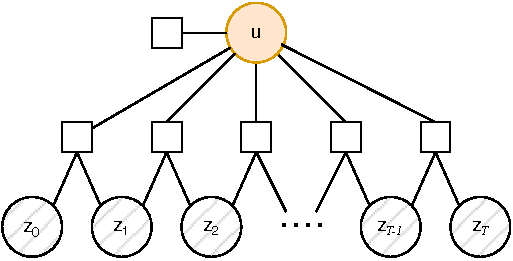
\includegraphics{FG_ts.drawio.pdf}
    \caption{Factor graph  for the generating equations of \eqref{eq:ts-sem}}
    \label{fig:ts_fg}
\end{figure}

% \subsection{Noisy observations}
% For exposition in this paper, we have assumed that we observe realisations of the series noiselessly.
% More generally, we might observe some noisy linear function of the true target values.
% \begin{align*}
%     \state_{t}&=\op{P}(\state_{\tm}, \forcing),\quad t=1, 2, \cdots, T\\
%     \outp_{t}&=\op{Y}\state_{t},\quad t=1, 2, \cdots, T\numberthis\label{eq:ts-sem-noisy}
% \end{align*}\nb{missing priors}
% where our observations are actually of \(\outp_{t}=\outpst_{t}\).
% Then the associated factor graph is more complicated (Figure~\ref{fig:ts_fg_noisy}) and the inference procedure is in fact loopy belief propagation.
% In this case we need to solve the filtering problem, estimating \(\{\state_{t}\}_t\) from \(\{\outp_{t}\}_t\).
% The message-pasing schedule in this case is loopy, and may not converge, although the ensemble updates are well-defined under the assumption that our ensemble statistics are.
% \begin{figure}
%     \centering
%     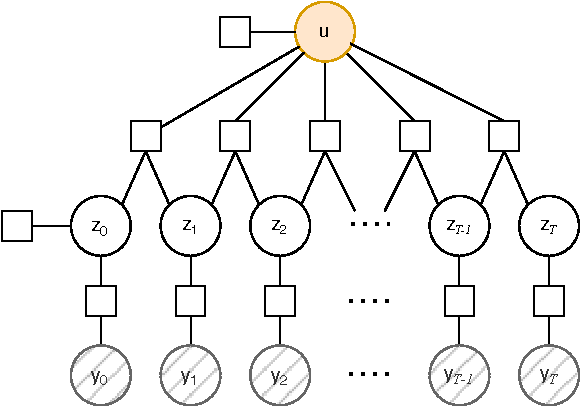
\includegraphics{FG_ts_noisy.drawio.pdf}
%     \caption{Factor graph for the generating equations of \eqref{eq:ts-sem-noisy}}
%     \label{fig:ts_fg_noisy}
% \end{figure}

% \section{Stationary moves in an ensemble Gaussian posterior}
% \subsection{Elliptical slice sampling}
% \subsection{Langevin}
% Suppose \(\vrv{x}\) is a  \(d\)-dimensional Gaussian RV
% \begin{align*}
% \vrv{x}&\sim\mathcal{N}(\overline{m}_{x}, \mm{K}_{\vrv{x}\vrv{x}})
% \end{align*}
% whose moments are  chosen to match the empirical moments of an ensemble \(\mm{X}=\begin{bmatrix}
%     \vrv{x}^{(1)} & \cdots & \vrv{x}^{(N)}
% \end{bmatrix}\) of iid samples
% so that
% \begin{align*}
% \overline{m}_{\vrv{x}}&:=\frac{1}{N}\sum_{i=1}^N \tilde{\vrv{x}^{(i)}}\\
% \mm{K}_{\vrv{x}\vrv{x}} &:= \breve{\mm{X}} \breve{\mm{X}}^{\top}\\
% \breve{\mm{X}}&=\frac{1}{\sqrt{N-1}}\begin{bmatrix}
%     (\vrv{x}^{(1)}-\overline{m}_{\vrv{x}}) & \cdots & (\vrv{x}^{(N)}-\overline{m}_{\vrv{x}})
% \end{bmatrix}\\
% \end{align*}
% Note that that the deviation matrix represents a square-root factorisation for the covariance, we can simulate new realisations from the distribution of this variable using
% \(\rv{x}\sim{m}_{\vrv{x}} + \breve{\mm{X}}\xi\) for \(\xi\sim\mathcal{N}(\vv{0}, \mm{I})\).
% A corollary to this is that this distribution and its updates comprise linear combinations of members of the ensemble, and so if \(d>N\) it cannot span the space of all possible realisations.\nb{not quite. what does it actually imply?}

% We could diversify the ensemble, in the sense of simulating realisations with the same moments but which did not come from the span of the ensemble if there existed a non-trivial random transform \(j\) which was not restricted to the span of this basis such that \(\vrv{x}\sim \dist{N}({m}_{\vrv{x}},\mm{K}_{\vrv{x}})\Rightarrow j(\vrv{x}) \disteq \vrv{x}\).
% Can we construct such a \(j\)?

% Langevin dynamics might be a tractable approach.
% Given \(\vrv{z}\sim\mathcal{N}(0,\mm{I}_{d})\) and a step size \(\epsilon\), an Euler-Maruyama approximation to a Langevin move is
% \begin{align*}
% j(\vv{x})
% &:= \vv{x}
% + \epsilon \nabla_{\vv{x}} \log p_{\vrv{x}}(\vv{x})
% + \sqrt{2\epsilon}~\vrv{z},\text{ and}\\
% \nabla_{\vv{x}} \log p_{\vrv{x}}(\vv{x})
% &=-( \vv{x}-{m}_{\vrv{x}})^{\top}\mm{K}_{\vrv{x}\vrv{x}}^{-1}
% \end{align*}
% thus
% \begin{align*}
% \Delta\vv{x} - \sqrt{2\epsilon}~ \vrv{z}
% &=\epsilon ( \vv{x}-{m}_{\vrv{x}})^{\top}\mm{K}_{\vrv{x}\vrv{x}}^{-1} \\
% (\Delta\vv{x} - \sqrt{2\epsilon}~ \vrv{z})\mm{K}_{\vrv{x}\vrv{x}}
% &=\epsilon ( \vv{x}-{m}_{\vrv{x}})^{\top}.
% \end{align*}
% Can we find any cool simplifications by plugging in ensemble deviations?
% Let us try:
% \begin{align*}
% \Delta\vv{x} - \sqrt{2\epsilon}~ \vrv{z}
% &=\epsilon ( \vv{x}-{m}_{\vrv{x}})^{\top}(\breve{\mm{X}} \breve{\mm{X}}^{\top})^{-1} \\
% (\Delta\vv{x} - \sqrt{2\epsilon}~ \vrv{z})\breve{\mm{X}} \breve{\mm{X}}^{\top}
% &=\epsilon ( \vv{x}-{m}_{\vrv{x}})^{\top} \\
% \Delta\vv{x}
% &=\epsilon ( \vv{x}-{m}_{\vrv{x}})^{\top}(\breve{\mm{X}} \breve{\mm{X}}^{\top})^{-1} + \sqrt{2\epsilon}~ \vrv{z}
% \end{align*}
% We can batch this, in which case
% \begin{align*}
% \Delta\mm{X}
% &=\epsilon (N-1) \breve{\mm{X}}^{\top}(\breve{\mm{X}} \breve{\mm{X}}^{\top})^{-1} + \sqrt{2\epsilon}~ \vrv{Z}\\
% \Delta\mm{X}  - \sqrt{2\epsilon}~ \vrv{Z} &=\epsilon (N-1) \breve{\mm{X}}^{\top}(\breve{\mm{X}} \breve{\mm{X}}^{\top})^{-1}
% \end{align*}

% This Euler-Maruyama approximation will clearly be bad if \(\epsilon\) is not tiny; we could consider implicit steps or Metropolis adjustment?
% Both those look expensive.

% We expect that iterating such steps will not be truly stationary; in the end the posterior covariance will drift.

% \section{Epistemic uncertainty in the ensemble posterior}\label{sec:u-uncertainty}

% Consider a jointly Gaussian ensemble covariance which includes a term to inflate the uncertainty of  our estimate of the posterior, because, e.g., we would like to decrease the confidence of our estimate convinced that it is \emph{truly} Gaussian, and quantifying that by adding Gaussian noise is the laziest option that might work.
% (Student-t distributions look hard and boring).
% This model looks similar to \eqref{eq:discrete_joint_enkf_sim} but with the uncertainty term moved:
% \begin{align*}
% \left.\left[\begin{array}{c}
%     \state_{t} \\
%     \forcing
% \end{array}\right]\right|\state_{\tm}
% &\simeq\dist{N}\left(
%     \left[\begin{array}{c}
%         \overline{\statest}\\
%         \overline{\forcingst}
%     \end{array}\right],
%     \left[\begin{array}{cc}
%         \breve{\mm{Z}}\breve{\mm{Z}}^{\top}
%         & \breve{\mm{U}}\breve{\mm{Z}}^{\top} \\\ % 3 backslashes or it breaks for some reason
%         \breve{\mm{Z}}\breve{\mm{U}}^{\top}
%         & \breve{\mm{U}}\breve{\mm{U}}^{\top} +\mm{K}_{\xi}
%     \end{array}\right]\numberthis\label{eq:discrete_joint_enkf_sim_misfit}
% \right).
% \end{align*}
% % What does that look like in ensemble inference?

% % \subsection{Adding independent noise to the samples}

% Simplest options:
% We can add some noise to each of the samples \(\forcingst^{(i)}\gets\vrv{\xi}^{(i)}\sim\mathcal{N}(0,\mm{K}_{\xi}).\)
% Is this well posed?
% How about if \(\mm{K}_{\xi}=\tau^2\mm{I}\)?
% Connection to Langevin sampling above.

% \subsection{Inflating posterior covariance}

% According to \citep{RothEnsemble2017} this is called variance inflation and is discussed in the literature.

% Alternatively, suppose the posterior ensemble has covariance  \(\breve{\mm{U}}\breve{\mm{U}}^{\top}\) but we wish it had covariance \(\breve{\mm{U}}'\breve{\mm{U}}'{}^{\top} \succ\breve{\mm{U}}\breve{\mm{U}}^{\top}\).
%
% We could change that by scaling the ensemble, possibly randomly, about the mean by some scalar (?) inflation factor \(\rv{s}\), \(\Ex\rv{s}>1\),
% \(\forcingst^{(i)}\gets\rv{s}(\forcingst^{(i)}-m_{\forcing})\) or even
% \(\forcingst^{(i)}\gets\vrv{S}(\forcingst^{(i)}-m_{\forcing})\) from some matrix-valued \(\vrv{S}\).

% Hmm, products of RVs is a complicated world to be in; I think I vote for deterministic scaling, or additive Gaussian noise, now that I think about it.

% \section{Ensemble Bayesian inversion 1: by pathwise GP sampling and error propagation}
% Here is a bad way of solving this problem because NN people always need to try the Jacobian first.

% Rather than assuming a jointly Gaussian distribution for all variables as in \eqref{eq:gaussian_approx_proc}, we make the weaker assumption that \emph{conditional on some fixed sample \(\state_{\tm}{=}\statest_{\tm}\), \(\state_{t}{=}\statest_{t}\) and \(\forcing\)} are jointly Gaussian with a conditional variance given by a local first-order Taylor expansion about \(\forcing{=}\forcingst\).
% That is, at pair \((\forcing, \state_{\tm})=(\forcingst, \statest_{\tm})\), the linearised joint distribution is
% \begin{align*}
%     {m}_{\forcing}
%         &=\proj_{\vv{X}}\forcing \numberthis\label{eq:mvn-m-inp}\\
%     {m}_{\state_{t}}
%         &=\proj_{\vv{S}}[\op{P}(\statest_{\tm},\forcingst)]\numberthis\label{eq:mvn-m-state}\\
%     \mm{K}_{\state_{t}\state_{t}}
%          &=J_{\forcingst}\mm{K}_{\forcing\forcing}J_{\forcingst}^{\top} +\sigma^2\mm{I}\numberthis \label{eq:discrete_pred_cov_taylor_local}\\
%     \mm{K}_{\state_{t}\forcing}
%     %     &= [\vv{k}_{\state_{t}\forcing}(s_i,x_j)]_{ij} \\
%     % \mm{K}_{\statest\forcingst}{}
%         &=\mm{K}_{\forcing\forcing}J_{\forcingst}^{\top}\numberthis
% \end{align*}
% where \(J_{\forcingst}:=\nabla_{\forcingst'}\proj_{\vv{S}}\op{P}(\statest_{\tm},\forcingst)\in\mathbb{R}^{|S|}\times\mathbb{R}^{|X|}\) is the Jacobian matrix of the projection of the forward predictor at this point.
% This rule gives us a different update \emph{for each sample} based on a different local linearisation.

% The Matheron update analog to \eqref{eq:pathwise-update} in such a model is thus
% \begin{align*}
% &(\tilde{{\forcing}} \gvn \state_{t}{=}\statest_{t},\state_{\tm}) \\
% &\disteq
% \tilde{{\forcing}}+\mm{K}_{\state_{t}\forcing} \mm{K}_{\state_{t}\state_{t}}^{-1}\left(\statest_{t}-{m}_{\state_{t}}\right)\\
% &=\tilde{{\forcing}}+\mm{K}_{\forcing\forcing}J_{\forcingst}^{\top} (J_{\forcingst}\mm{K}_{\forcing\forcing}J_{\forcingst}^{\top} +\sigma^2\mm{I})^{-1}\left(\statest_{t}-{m}_{\state_{t}}\right).\numberthis\label{pathwise-update-mc}
% \end{align*}
% This method has various apparent difficulties.
% % For one, the matrix inversion required by the update step \eqref{eq:pathwise-update} is an \(\mathcal{O}(|X||S|^3)\) operation.
% Under the discretisation \eqref{eq:discrete_joint_naive}, calculating the update \eqref{eq:discrete_pred_cov_taylor_local} naively is a \(\mathcal{O}(|X|^3|S|)\) operation since we need to invert  \(\mm{K}_{\forcing\forcing})\) to calculate it.
% Although this method has relaxed some assumptions of the Gaussian variational posterior approximation, it is even less computationally tractable; each sample update requires both the covariance inversion and the calculation of a different local Jacobian matrix.

% Ensemble Kalman methods~\cite{EvensenData2009} empirically approximate intractably large covariance matrices \(\mm{K}_{\forcing\forcing}\), e.g.\ in \eqref{eq:pathwise-update} where we need to find an update.

% Then,
% \begin{align*}
% &\mm{K}_{\forcing\forcing}J_{\forcingst}^{\top} (
%     J_{\forcingst}\mm{K}_{\forcing\forcing}J_{\forcingst}^{\top}
%     +\sigma^2\mm{I}
%     )^{-1}\\
% % &=\frac{1}{\sigma^2}(
% %     \mm{K}_{\forcing\forcing}^{-1} + \frac{1}{\sigma^2} J_{\forcingst}^{\top}J_{\forcingst}
% %     )^{-1}J_{\forcingst}^{\top}\\
% &\simeq\breve{\mm{U}}\breve{\mm{U}}^{\top}J_{\forcingst}^{\top} (
%     J_{\forcingst}\breve{\mm{U}}\breve{\mm{U}}^{\top}J_{\forcingst}^{\top}
%     +\sigma^2\mm{I}
%     )^{-1}\\
% &=\underbrace{\breve{\mm{U}}}_{|X|\times N} \left(
%         \underbrace{\breve{\mm{U}}^{\top}}_{N\times |X|}
%         \underbrace{J_{\forcingst}^{\top}}_{|X|\times |S|}
%         \underbrace{J_{\forcingst}}_{|S|\times |X|}
%         \underbrace{\breve{\mm{U}}}_{|X|\times N}
%         +\frac{1}{\sigma^2}\mm{I}
%     \right)^{-1}
%     \underbrace{\breve{\mm{U}}^{\top}}_{N\times |X|}
%     \underbrace{J_{\forcingst}^{\top}}_{|X|\times |S|}
% \end{align*}
% Another useful one is the Kalman gain,
% \begin{align*}
% \mm{G} &:=\mm{K}_{\forcing\forcing}J_{\forcingst}^{\top} (J_{\forcingst}\mm{K}_{\forcing\forcing}J_{\forcingst}^{\top} +\sigma^2\mm{I})^{-1}\\
% \underbrace{\mm{G}}_{|X|\times |S|} &:=
%     \underbrace{\breve{\mm{U}}}_{|X|\times N}
%     \underbrace{J_{\forcingst}^{\top}}_{|X|\times |S|}
%     \left(
%         \underbrace{J_{\forcingst}}_{|S|\times |X|}
%         \underbrace{\breve{\mm{U}}}_{|X|\times N}
%         \underbrace{\breve{\mm{U}}^{\top}}_{N \times |X|}
%         \underbrace{J_{\forcingst}^{\top}}_{|X| \times |S|}
%         +\sigma^2\mm{I}
%     \right)^{-1}
% \end{align*}
% which we can calculate by solving for
% \begin{align*}
% \mm{G}\left(J_{\forcingst}\breve{\mm{U}}\breve{\mm{U}}^{\top}J_{\forcingst}^{\top} +\sigma^2\mm{I}\right) &:=\breve{\mm{U}}\breve{\mm{U}}^{\top} J_{\forcingst}^{\top}
% \end{align*}
% % or using Welling's variant Woodbury:
% % If \(\mathbf{P}, \mathbf{R}\) are positive definite, then
% % \begin{align*}
% %     \mathbf{P} \mathbf{B}^{\top}\left(\mathbf{B} \mathbf{P} \mathbf{B}^{\top}+\mathbf{R}\right)^{-1}
% %     =\left(\mathbf{P}^{-1}+\mathbf{B}^{\top} \mathbf{R}^{-1} \mathbf{B}\right)^{-1} \mathbf{B}^{\top} \mathbf{R}^{-1}
% % \end{align*} from which
% % \begin{align*}
% %     &(\breve{\mm{U}}^{\top}\breve{\mm{U}}) J_{\forcingst}^{\top}\left(J_{\forcingst} (\breve{\mm{U}}^{\top}\breve{\mm{U}}) J_{\forcingst}^{\top}+(\sigma^2\mm{I})\right)^{-1}\\
% %     &=\frac{1}{\sigma^2}\left((\breve{\mm{U}}^{\top}\breve{\mm{U}})^{-1}+\frac{1}{\sigma^2}J_{\forcingst}^{\top}  J_{\forcingst}\right)^{-1} J_{\forcingst}^{\top}
% % \end{align*}
% which is not \emph{prima facie} a huge saving, although we can group the \(\underbrace{J_{\forcingst}}_{|S|\times |X|}\underbrace{\breve{\mm{U}}}_{|X|\times N}\) terms.

% \section{Design}
% a.k.a. choosing projections.

% We largely ignore the question of optimal placement of observation in the current work.
% Optimal \(\set{S}\)~\cite{AlexanderianOptimal2021}?
% Optimal \(\Phi\)~\cite{LassasDiscretizationinvariant2009}?

% What do we actually converge to if we try to update th whole thing using low-dim projections?

% The unfavourable scaling is in the output observation term, so we now have a question about how big to make that. There are some results in subsampling covariance observations that we possibly need to digest to manage this term \cite{ChenStochastic2020,MinhFinite2022}.

% \section{Offcut: Posterior updates by random projections}

% Can we make site updates of posterior fields cheaper by updating random projections of the field in some sense?

% As seen in sliced Fisher score matching.
% Is that a way of doing partial updates?

% \section{Offcut: inversion by Newton methods}
% \cite{WilkinsonBayesNewton2021}

% \subsubsection{by that weird Laplace-on-a-graph trick the opposition uses}
% \cite{MagnaniApproximate2022}

% \subsection{Robust losses}

% \cite{DavisonFutureMapping2019,DonohoHigh2013}
\fi

\iffalse
\russ{Is this still in progress?}\danm{yes, omg, I just realised it doesn't make sens for the linearised case for one thing.}
\russ{I can't find the definition of $\vrv{\nu}_t$ or $\hat{p}$.}\danm{  $\vrv{\nu}_t$ is \eqref{eq:ts-sem-stoch}, $\hat{p}$ needs a do-over for new notation. what do we call an estiamte of a realisation lieklihood now?}
\russ{There is an object $\rho(\forcingst \gvn \mathcal{D}_{t-1})$ which is the evaluation of the likelihood conditioned on the observations. Is that what you are looking for? Or are you looking for something like $\rho(\forcingst \gvn \mathcal{D}_t, \state_t)$? Not sure what ``estimate'' means or ``realisation'' in this context}
\russ{ Do we really want to compute an expectation over $\forcing$?}
\danm{yes, as it stands, but these is a weirdness in the problem framing that leads to that yes; we are using the true prior as the generating process for the data here. Generally in stats want to randomise over all data-generating processes, but not over all realisations from the prior. There are two things wrong there; 1) knowing the true prior distribution fro everything is sus 2) in fact we want to average over all possible inference steps, which includes taking expectations over all possible posterior updates to all possible priors, which is a hard integral and in any case does not do quite what we want, since a given inference step does not ``know'' if it is early or late in the inference process.}
We have free hyperparameters in both the linearised and ensemble methods.
In the evidence framework, we would like to choose hyperparameters \(\sigma^2\) and \(\tau^2\) to maximise some notion of the expected quality of inference over all data.
For example, for a given inference method, operator \(\op{P}\) and distributions \(\Law(\forcing),\Law(\state_{0}),\{\Law(\vrv{\nu}_{t}\}_t\), we might maximise the expected likelihood of observations drawn from these distributions,
\begin{align*}
    &\Ex_{\forcing, \state_{0}, \{\vrv{\nu}_t\}_t} [\widehat{p}(\forcing\gvn \state_{0},\dots\state_{T})]\\
\end{align*}
The deficiency of solving this problem directly is that it requires us to estimate high-dimensionalintegrals at potentially high computational cost.

In practice we have a cheaper approximate alternative:
Maximum likelihood over residuals is consistent for estimating the model noise terms~\citep{MitchellAdaptive2000} and the maximum likelihood estimate of both \(\sigma^2\) and \(\tau^2\) is simply the variance of the model residuals which does not require calculating or optimising over the model density directly.
In practice we estimate both of these terms by evaluating the method over artificial data from simulator runs with new random seeds.
\fi


% Addressing the difficulties this imposes is studied in the Ensemble Kalman literature (see e.g.~\cite{FearnheadParticle2018} and references therein).
% One pragmatic means of allowing the model to span a wider space, which we exploit in this work, is to inject additional element-wise i.i.d. noise to each member of the ensemble, \(\forcing_{t}^{(i)}{}'=\forcing_{t}^{(i)}+\dist{N}(\vv{0},\kappa^2\mm{I})\).
% \danm{In fact the optimal \(\kappa\) is 0 by the obvious methods; could delete?}

% Plugging in sample covariances of~\eqref{eq:discrete_joint_enkf_sim} to the  Matheron update~\eqref{eq:pathwise-update}, we need to solve an inner problem
% \begin{align*}
% &(\tilde{{\forcing}}^{(i)} \gvn \state_{t}{=}\statest_{t},\state_{\tm}) \\
% &\disteq
% \tilde{{\forcing}}^{(i)}+\mm{K}_{\state_{t}\forcing} \mm{K}_{\state_{t}^{(i)}\state_{t}^{(i)}}^{-1}\left(\statest^{(i)}-\statest_{t}\right)\\
% &=\tilde{{\forcing}}^{(i)}+\breve{\mm{U}}\breve{\mm{Z}}^{\top}(\breve{\mm{Z}}\breve{\mm{Z}}^{\top} + \sigma^2\mm{I})^{-1}\left(\statest^{(i)}-\statest_{t}\right)
% \numberthis\label{eq:pathwise-update-ensemble-sim}\\
% &=\tilde{{\forcing}}^{(i)}
% +\underbrace{\breve{\mm{U}}}_{|X|\times N}
% \underbrace{\breve{\mm{Z}}^{\top}}_{N\times |S|}{(
%   \underbrace{\breve{\mm{Z}}}_{|S|\times N}
%   \underbrace{\breve{\mm{Z}}^{\top}}_{N\times |S|} + \sigma^2\mm{I}
% )}^{-1}\left(\statest^{(i)}-\statest_{t}\right).
% \end{align*}

% At first glance, this method still requires an intractably expensive \(\mathcal{O}(D_{\vrv{\state}}^3)\) cost when solving systems involving the  covariance \((\breve{\mm{Z}}\breve{\mm{Z}}^{\top} + \sigma^2\mm{I})\) in \eqref{eq:pathwise-update-ensemble-sim}.
% However, the empirical representation has structure we can exploit to approximate its solution efficiently via Lanczos decomposition.
% That trick is known in the Gaussian process literature in the context of Lanczos Variance Estimates (LOVE)~\citep{PleissConstantTime2018}, %\nb{TODO; check if this is well known in EnKF? Surely. what do they call it?}
% although we exploit it in a different manner.

% Given some rank \(k\) and an arbitrary starting vector \(\vv{b}\), the Lanczos algorithm iteratively approximates  \(\mm{A} \in\mathbb{R}^{n \times n}\) by a low rank factorisation \(\mm{A}\approx \mm{Q} \mm{T} \mm{Q}^{\top}\), where \(\mm{T} \in \mathbb{R}^{k \times k}\) is tridiagonal and \(\mm{Q} \in \mathbb{R}^{n \times k}\) has orthogonal columns.
% Crucially, we do not need to form \(\mm{A}\) to evaluate matrix vector products \(\mm{A}\vv{b}\) for arbitrary vector \(\vv{b}\).
% \nb{accuracy of this update? Depends on condition number}
% Moreover, with a given Lanczos approximand \(\mm{Q},\mm{T}\) we may estimate
% \begin{align*}
% \mm{A}^{-1}\vv{c}\approx \mm{Q}\mm{T}^{-1}\mm{Q}^{\top}\vv{c}.\numberthis\label{eq:lanczos-inv}
% \end{align*}
% even for \(\vv{b}\neq\vv{c}\).\nb{citation chase for bounds on this approx quality.}

% In \eqref{eq:pathwise-update-ensemble-sim} we must calculate
% %\nb{Dan M to fix this bit - I think it was supposed to be Zs and also we agreed that this needs rewording - I was confused what you were "solving" here}
% \(\left(\breve{\mm{Z}} \breve{\mm{Z}}+\sigma^2 \mm{I}\right)^{-1}\left(\statest^{(i)}-\statest_{t}\right)\).
% We approximate the solution to this linear system using the partial Lanczos decomposition starting with probe vector \(\vv{b}=\tilde{m}_{\statest}\) and \(\mm{A}=\left(\breve{\mm{U}} \breve{\mm{U}}+\sigma^2 \mm{I}\right)\).
% % Applying the approximation in an ensemble  context in \meth{} exploits the square-root decomposition of the variance in terms of deviance matrices.
% This requires \(k\) matrix vector products of the form %\nb{this should be two equations - not two equal signs on the same line.}
% \begin{align*}
% \underbrace{\left(\underbrace{\breve{\mm{U}} \breve{\mm{U}}^{\top}}_{\mathcal{O}(ND_{\vrv{\state}}^2)}+\sigma^2 \mm{I}\right)\vv{b}}_{\mathcal{O}(D_{\vrv{\state}}^2)}
% =\underbrace{\breve{\mm{U}} \underbrace{(\breve{\mm{U}}^{\top}\vv{b})}_{\mathcal{O}(ND_{\vrv{\state}})}}_{\mathcal{O}(ND_{\vrv{\state}})} +\sigma^2 \vv{b}.
% \end{align*}
% Using the latter representation, the required matrix-vector product may be found with a time complexity cost of \(\mathcal{O}(ND_{\vrv{\state}})\).
% Space complexity is also \(\mathcal{O}(ND_{\vrv{\state}})\).
% The output of the Lanczos decomposition is \(\mm{Q},\mm{T}\) such that \(\left(\tilde{\mm{K}} +\sigma^2 \mm{I}\right)\vv{b}\approx \mm{Q} \mm{T} \mm{Q}^{\top}\vv{b}\), i.e. a low rank approximation of the covariance-matrix-vector product.
% Then, by~\eqref{eq:lanczos-inv}, the solution to the inverse-covariance-matrix-vector product may be approximated by
% \(\left(\tilde{\mm{K}} +\sigma^2 \mm{I}\right)^{-1}\left(\statest^{(i)}-\statest_{t}\right)\approx \mm{Q}\mm{T}^{-1}\mm{Q}^{\top}\left(\statest^{(i)}-\statest_{t}\right)\), requiring the solution in \(\mm{x}\) of the much smaller linear system \(\mm{X}\mm{T}=\mm{Q}\).
% Exploiting the positive-definiteness of \(\mm{T}\) we may use the Cholesky decomposition of \(\mm{T}=\mm{L}^{\top}\mm{L}\) for a constant speedup over solving an arbitrary linear system.
% The time cost of the solution is \(\mathcal{O}(D_{\vrv{\state}}k^3)\), for an overall cost to the matrix inversions of \(\mathcal{O}(ND_{\vrv{\state}}k+D_{\vrv{\state}}k^3)\).
% \nb{make more precise; i think we have missed some multiplies and Lanczos overhead, plus deviation calcs; also if we use iterative matheron, how many steps do we take in general?}


\iffalse
The Matheron update maps marginal Gaussian samples to conditional Gaussian samples.
In particular, if  \begin{align*}
    \begin{bmatrix}\vrv{y}\\ \vrv{w}
\end{bmatrix}\sim\mathcal{N}\left(\begin{bmatrix}
    m_{\vrv{y}}\\ m_{\vrv{w}}
\end{bmatrix},\begin{bmatrix}
    \mm{K}_{\vrv{y}\vrv{y}} & \mm{K}_{\vrv{y}\vrv{w}} \\
    \mm{K}_{\vrv{w}\vrv{y}} & \mm{K}_{\vrv{w}\vrv{w}}
\end{bmatrix}\right),
\end{align*}
then
\begin{align*}
\vrv{y}+\mm{K}_{\vrv{w}\vrv{y}} \mm{K}_{\vrv{w}\vrv{w}}^{-1}\left[\vrv{w}-{m}_{\vrv{w}}\right]\disteq
    \left(\vrv{y}\gvn \vrv{w}=\vv{w}\right),
\end{align*}
and this update may be applied sample-wise to the members of the ensemble.
%For further details see Appendix~\ref{app:matheron}.
In \meth{}, we substitute the empirical moments into the Matheron update formula to construct sample-wise updates to the ensemble members as
\fi

\iffalse
\begin{align*}\left.
\left[\begin{array}{c}
    \statest_{t}^{(i)} \\
    \forcingst^{(i)}
\end{array}\right] \right| \mathcal{D}_{t-1}
    &\sim \dist{N}\left(
    \left[\begin{array}{c}
        \overline{\mm{Z}}_{t}\\
        \overline{\mm{U}}_{\tm}
    \end{array}\right],
    \left[\begin{array}{cc}
        \breve{\mm{Z}}_{t}\breve{\mm{Z}}_{t}^{\top} +\sigma^2\mm{I}
        & \breve{\mm{U}}_{\tm}\breve{\mm{Z}}^{\top}_{t} \\\ % 3 backslashes or it breaks for some reason
        \breve{\mm{Z}}_{t}\breve{\mm{U}}_{\tm}^{\top}
        & \breve{\mm{U}}_{\tm}\breve{\mm{U}}_{\tm}^{\top} + \tau^2\mm{I}
    \end{array}\right]\right)\numberthis\label{eq:discrete_joint_enkf_sim}%\\
    % &=:\dist{N}\left(
    % \left[\begin{array}{c}
    %     \overline{\mm{Z}}_{t}\\
    %     \overline{\mm{U}}_{\tm}
    % \end{array}\right],
    % \left[\begin{array}{cc}
    %     \mm{K}_{\mm{ZZ},t}
    %     & \mm{K}_{\mm{UZ},t} \\
    %     \mm{K}_{\mm{ZZU},t}
    %     & \mm{K}_{\mm{UU},\t}
    % \end{array}\right]\right).
\end{align*}
\fi


\end{document}